\newcommand{\aref}[1]{\autoref{#1}\space}
\renewcommand{\algorithmcfname}{算法}
\chapter{绪论}
\section{研究背景与意义}
机器人一直是人类孜孜不倦探索钻研的目标,人类一直致力于实现让机器人覆盖人
类的功能,使人类从繁杂重复的体力劳动中或是危险系数较高的工作中解放出来。将机
器人按照驱动方式区分可以分为轮履式机器人与腿足式机器人,就当今已存在的机器人
中,轮式机器人和履带式机器人要占据绝大部分。这种类型机器人有着移动快,控制简
单,实现方便的特点,同时在平坦以及硬质路面有着移动速度较快的特性。但是此类机
器人无法适应复杂路面,比如轮式机器人无法实现在阶梯或是崎岖路面前进,履带式机
器人也很难做到上下楼梯。相比较来说,腿足式机器人就能很好适应复杂路面,在崎岖
路面有着得天独厚的优势,从人类通过双腿可以适应自然界绝大部分的地貌环境就可以
看出来,足式机器人更适合于复杂的陆地环境\cite{schraft2000service}。人类通过视觉信息选取离散的落脚点
以跨过不同的障碍物和适应不同的路面,腿足式机器人可以通过步态规划以及身体平衡
控制做到不平整路面的前进,但目前仍然存在许多挑战。

另一方面,腿足式也是自然界大部分生物所采取的前进方式,所以机器人采用腿足
式方式能够更好的融入人类生活中。采用和人类相似的外形使得腿足式机器人相对于轮
式和履带式机器人在亲和力方面有着难以匹敌的优势,完美的适应人类的工作环境\cite{2010067776.nh}。
在未来利用仿人机器人取代人类在高危险环境下的工作或者重复性较高的体力劳动的
是必然趋势。此外对于腿足式机器人的研究还能够通过得到腿部运动的规律设计康复外
骨骼等助力工具帮助残疾人恢复健康。对于腿足式机器人的研究能够更好的了解人类腿
部运动机理,利用康复性外骨骼机器人帮助腿部残疾的患者恢复健康也是大势所趋。
目前国内外关于腿足式尤其是仿人机器人的研究也受到越来越多的关注,仿人机器
人是仿生机器人领域的代表之一,它集机械、电气、计算机、传感器等多种学科于一体,
是直接模仿采用仿人前进动物的一类机器人\cite{梶田秀司2007仿人机器人},而仿人机器人跑跳步态一直是腿足机器
人领域的重要挑战和研究热点之一。仿人机器人采用跑跳步态可以实现更为快速的运动
速度,由于机器人在空中相持续时间内还会因为惯性具有向前的速度,所以机器人的前
进速度就不再受到机器人连杆长度的限制,比采用行走的速度有了较大的提升。机器人
由行走切换为跑步,进一步释放机器人关节电机的性能,大大提高机器人运动的灵活性。
相对应的,机器人采用跑跳步态对于机器人的动态平衡控制提出更高的要求,需要机器
人在由空中相与支撑相的相互切换中迅速调整控制策略,施加精确的控制作用以使机器
人维持期望的运动速度和稳定状态。目前国内外仿人机器人实现跑跳步态的机器人还屈
指可数,这一领域将会是未来持续的研究方向。

\section{国内外研究现状介绍}
\subsection{日本仿人机器人研究现状}

早在20世纪60年代末,日本就开始了对仿人仿人机器人的研究。日本早稻田大学的Ichiro Kato教授于1969~1971年设计制作了液压驱动的
仿人机器人WL-3以及WL-5(\aref{subfig:wl5}),并以此为基础在1973年研制了仿人机器人WABOT-1 (\aref{subfig:wabot1}),这也被认为是最早的现代仿人机器人。
尽管这些机器人运动能力相当差,只能实现一些静态动作,但也在客观上引发了学术界和产业界对仿人仿人机器人研究的兴趣。

\begin{figure}[htbp]
    \centering
    \subcaptionbox{WL-5\label{subfig:wl5}}
        {%
            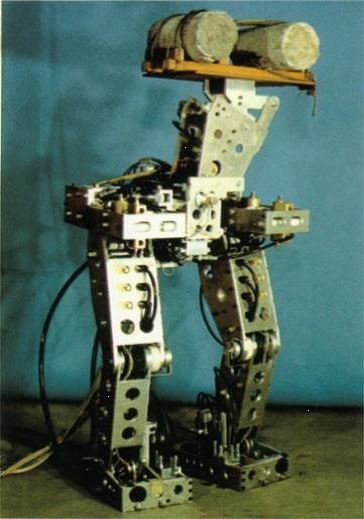
\includegraphics[height = .5\linewidth]{WL-5.jpg}}
    \subcaptionbox{WABOT-1\label{subfig:wabot1}}
        {%
            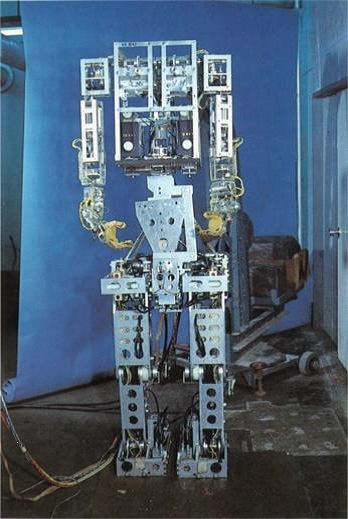
\includegraphics[height = .5\linewidth]{WABOT-1.jpg}}
    \caption{早稻田大学研制的早期仿人机器人\label{fig:japan_old}}
\end{figure}
\begin{figure}[htbp]
    \centering
    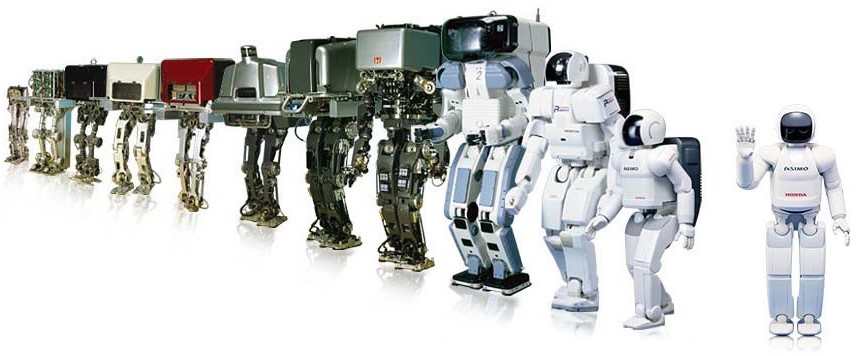
\includegraphics[width=1.\linewidth]{asimo.jpg}
    \caption{\label{fig:asimo}本田公司研制的ASIMO仿人机器人及其历代原型机}
\end{figure}

20世纪80年代,日本本田公司(Honda)也开始了仿人机器人的研究,出于控制方便和动力源可携带等方面的考虑,本田选择了电机驱动的技术路线,
经过E0到E6的七代步行样机研发,以及加入仿人上半身的P1到P2的原型机迭代,以及基于P系列原型机做出的小型化改进,终于在2000年推出了著名的
仿人机器人ASIMO(\aref{fig:asimo})。 ASIMO具有良好的外观设计,并且集成了视觉识别、语音交互等技术,是最为人所熟知的仿人机器人之一。
本田也不断地对ASIMO¬进行改进,到2011年时ASIMO的奔跑速度就达到了9km/h,并能完成上下台阶、倒水等展示任务\cite{Honda}。

\begin{figure}[htbp]
    \centering
    \subcaptionbox{HRP-1\label{subfig:HRP-1}}
        {%
            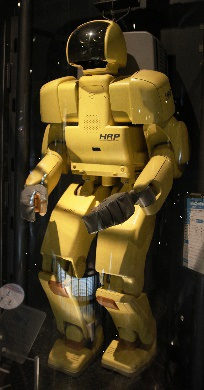
\includegraphics[height = .3\linewidth]{HRP-1.jpg}}
    \subcaptionbox{HRP-2\label{subfig:HRP-2}}
        {%
            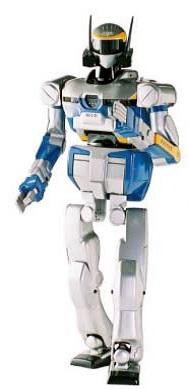
\includegraphics[height = .3\linewidth]{HRP-2.jpg}}
    \subcaptionbox{HRP-3\label{subfig:HRP-3}}
        {%
            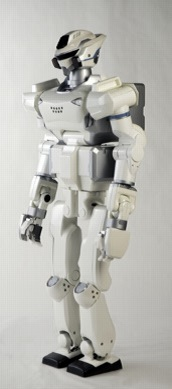
\includegraphics[height = .3\linewidth]{HRP-3.jpg}}

    \subcaptionbox{HRP3L-JSK\label{subfig:HRP3L-JSK}}
        {%
            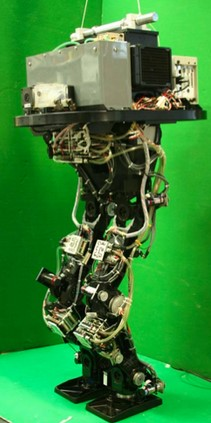
\includegraphics[height = .3\linewidth]{HRP3L-JSK.jpg}}   
    \subcaptionbox{HRP-4c\label{subfig:HRP-4c}}
        {%
            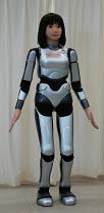
\includegraphics[height = .3\linewidth]{HRP-4c.jpg}}       
    \subcaptionbox{HRP-4\label{subfig:HRP-4}}
        {%
            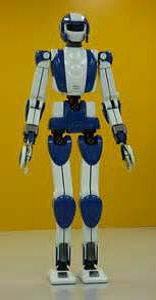
\includegraphics[height = .3\linewidth]{HRP-4.jpg}}       
    \subcaptionbox{HRP-5P\label{subfig:HRP-5P}}
        {%
            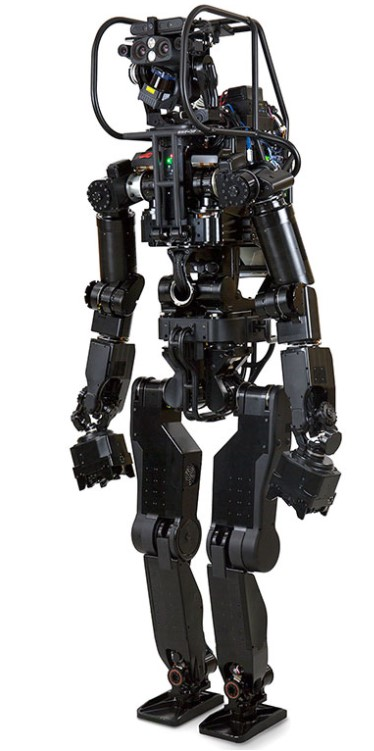
\includegraphics[height = .3\linewidth]{HRP-5P.jpg}}       

    \caption{HRP系列仿人机器人\label{fig:japan_hrp}}
\end{figure}

除ASIMO外,日本产业技术综合研究院也在1998年开启了仿人机器人项目(Humanoid Robotics Project, HRP),HRP系列(\aref{fig:japan_hrp})
也采取了电机位置伺服驱动的思路,2018年第五代最新的HRP-5P发布(\aref{subfig:HRP-5P})。HRP-5P高182cm,重101kg,搭载的视觉和激光传感器可以识别工具类别并灵活使用工具,
并且具备搬运木板等较重负载的能力\cite{HRP},体现了HRP系列仿人20多年的研究积累。

\begin{figure}[htbp]
    \centering
    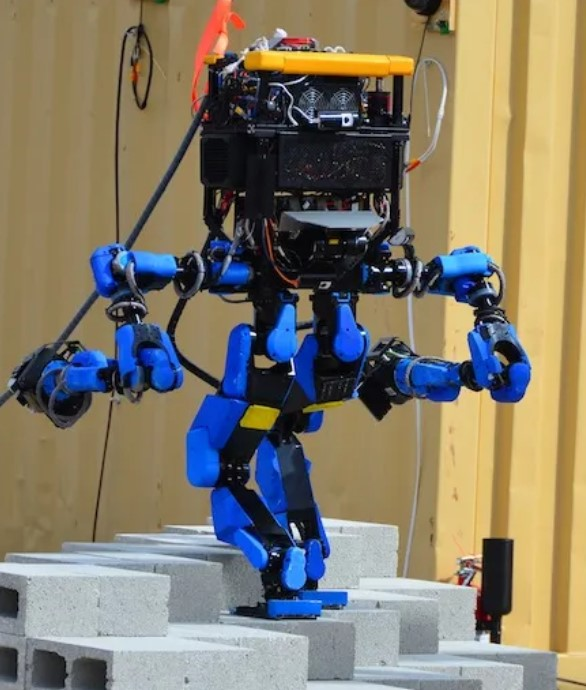
\includegraphics[height=.35\textwidth]{s-one1.jpg}
    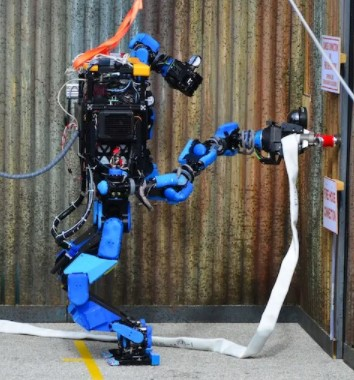
\includegraphics[height=.35\textwidth]{s-one2.jpg}
    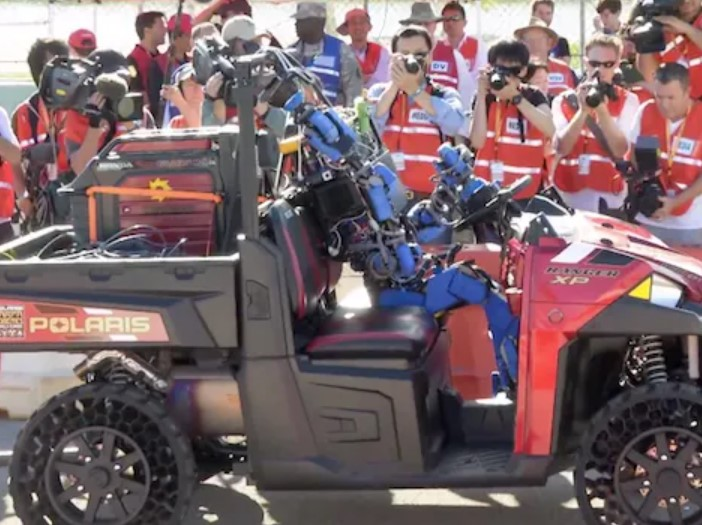
\includegraphics[width=.6\textwidth]{s-one3.jpg}
    \caption{\label{fig:s-one}S-One机器人完成DRC的各项任务}
\end{figure}

在参与HRP计划的研究机构中,东京大学的情报工学研究室(Johou Systems Kougaku Laboratory,简称JSK)取得的成果较为突出,2010年,JSK的Urata和Nakanishi
创造性地给伺服电机加入液冷系统,大大提高了电机的散热效率,再加上他们设计的大电流驱动器,整套驱动系统的功率密度得到了显著提升。
他们将改造过的驱动系统安装在了一对源于HRP-3的腿上从而得到了HRP3L-JSK(\aref{subfig:HRP3L-JSK}),HRP3L-JSK强大的驱动性能使其同时具有了快速运动和承受大负载的能力。
Urata等人之后创建SCHAFT公司,在HRP3L-JSK的基础上开发了S-One。搭载了强大驱动系统的S-One在DRC2013中成功完成了各项任务(\aref{fig:s-one}),以大比分优势取得了第一名,
SCHAFT也在2013年被Google收购。SCHAFT之后在2016年发布了其新研发的直线腿式仿人机器人,该机器人能够自主上下楼梯,并且能够在足底打滑的情况下快速恢复平衡\cite{SCHAFT}。

\subsection{美国仿人机器人研究现状}

从20世纪80年代开始,Marc Raibert及其领导的MIT腿机器人实验室(MIT LegLab)研发了一系列具备动态平衡及跳跃能力的腿足机器人。他们采取了由单腿到多腿,
由平面到三维的由简到繁递进的研究思路,利用压缩气体动力源高能量密度的优势,实现了即使放到今天也相当惊人的效果。1980至1982年他们研制了第一台跳跃机器人
Planar One-Leg Hopper(\aref{subfig:one-leg-2d}),该机器人由气缸驱动腿部的摆动和伸缩,可以实现平面约束下连续的稳定跳跃;在1983至1984年这个平面单腿机器人被拓展到了三维空间,
3D One-Leg Hopper(\aref{subfig:one-leg-3d})实现了在三维空间的连续稳定跳跃;1985至1990年间,Raibert又将平面单腿机器人拓展成为平面仿人机器人Planar Biped(\aref{subfig:biped-2d}),
实现了平面约束下的奔跑、越障、空翻等动作;后面Planar Biped 又进一步被拓展为3D Biped(\aref{subfig:biped-3d}),该仿人机器人能够在三维空间进行跑跳运动并完成空翻动作\cite{raibert1986legged}。

\begin{figure}[htbp]
    \centering
    \subcaptionbox{Planar One-Leg Hopper\label{subfig:one-leg-2d}}
        {%
            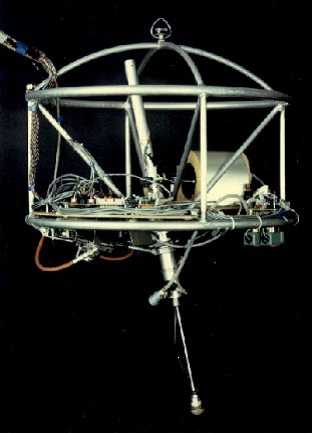
\includegraphics[height = .45\linewidth]{leglab1.jpg}}
    \subcaptionbox{3D One-Leg Hopper\label{subfig:one-leg-3d}}
        {%
            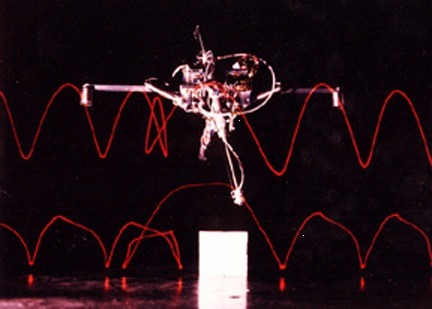
\includegraphics[height = .45\linewidth]{leglab2.jpg}}
    \caption{MIT LegLab 早期的单腿跳跃机器人\label{fig:leglab}}
\end{figure}
\begin{figure}[htbp]
    \centering
    \subcaptionbox{Planar Biped\label{subfig:biped-2d}}
        {%
            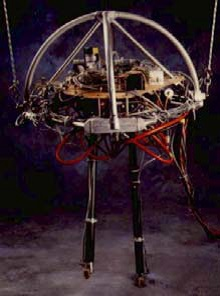
\includegraphics[height = .425\linewidth]{leglab3.jpg}}
    \subcaptionbox{3D Biped\label{subfig:biped-3d}}
        {%
            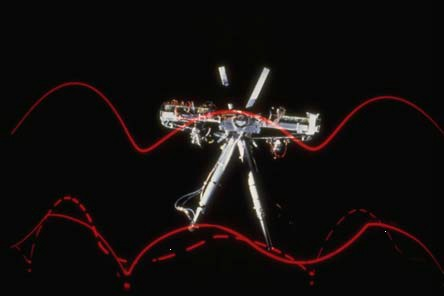
\includegraphics[height = .425\linewidth]{leglab4.jpg}}
    \caption{MIT LegLab 早期的仿人机器人\label{fig:leglab_biped}}
\end{figure}

此后Raibert离开MIT,创建了波士顿动力公司(Boston Dynamics)继续进行腿足机器人的相关研究。2009年,波士顿动力发布了新一代的仿人机器人PETMAN(\aref{fig:leglab_biped}),
PETMAN继承了MIT LegLab 时期的驱动思路,采用了同为流体驱动的液压驱动方案,它能模仿人的行走步态,并具有一定抗外界干扰的能力[8]。在PETMAN的基础上,
波士顿动力公司从2013年开始又进一步研发了Atlas,为其升级了动力系统,并增加了深度相机、激光雷达等传感器。Atlas被IHMC使用参加了DRC2015(\aref{fig:atlas})并取得了第二名。

\begin{figure}[htbp]
    \centering
    \subcaptionbox{PETMAN Prototype\label{subfig:biped-2d}}
        {%
            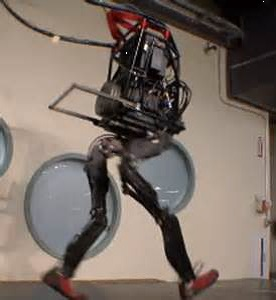
\includegraphics[height = .5\linewidth]{petman1.jpg}}
    \subcaptionbox{PETMAN\label{subfig:biped-3d}}
        {%
            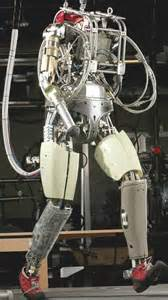
\includegraphics[height = .5\linewidth]{petman2.jpg}}
    \caption{波士顿动力公司研发的两代PETMAN样机\label{fig:leglab_biped}}
\end{figure}
\begin{figure}[htbp]
    \centering
    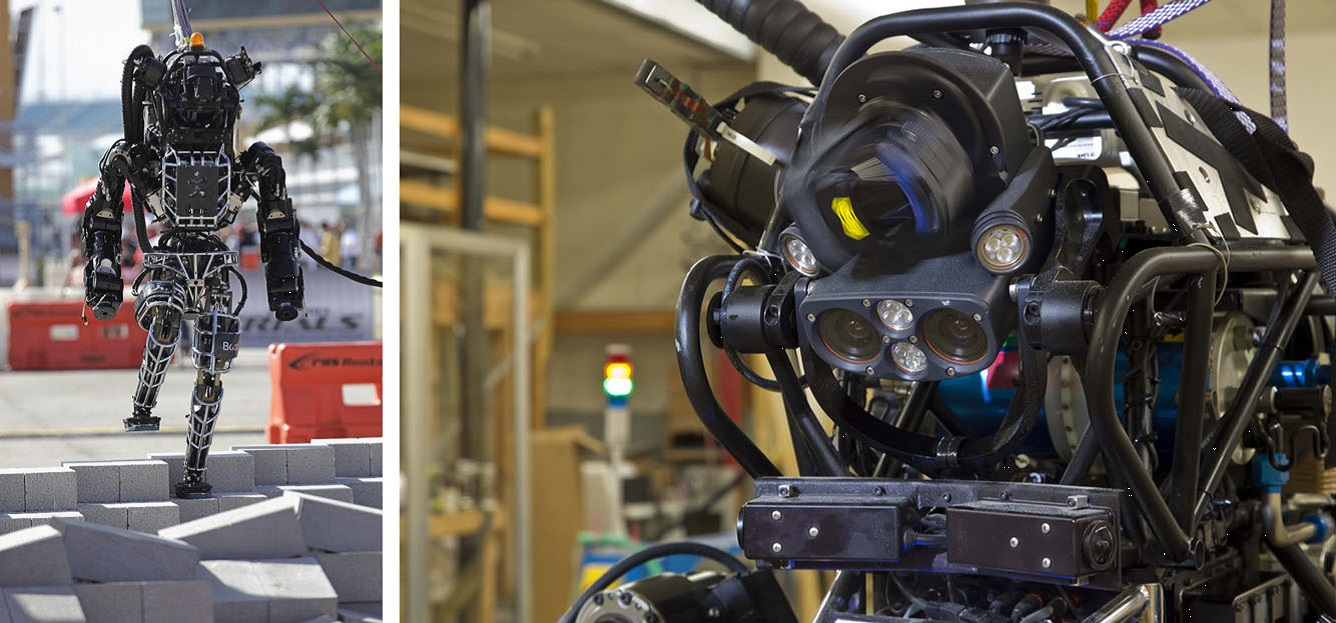
\includegraphics[height=.42\linewidth]{atlas.jpg}
    \caption{\label{fig:atlas}IHMC参加DRC2015使用的Atlas机器人}
\end{figure}

随后波士顿动力公司将Atlas进一步小型化,为其开发了人机协作搬运货物等功能。小型化的Atlas能够自带电池在野外复杂环境行走,不再依赖于实验室的理想环境。从2018年开始,
波士顿动力公司每年都会发布Atlas的最新进展,采取液压驱动方案的Atlas也被公认为是世界上最先进的仿人仿人机器人。到2021年,Atlas已经能够完成后空翻、高难度跑酷、
甚至是跳舞等各种复杂高动态动作(\aref{fig:atlas_dance}),目前其他所有公开的仿人仿人机器人都无法在运动能力上望其项背。

\begin{figure}[htbp]
    \centering
    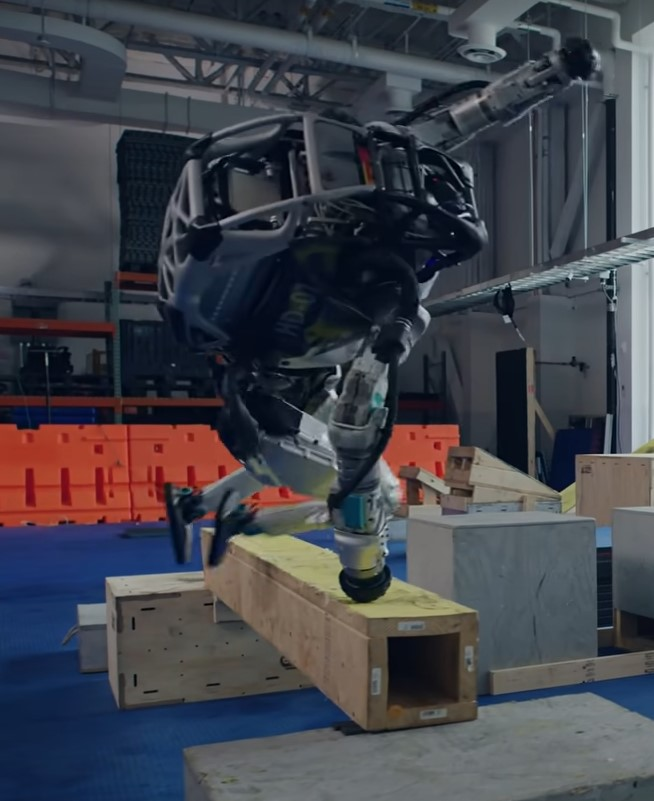
\includegraphics[height=.43\linewidth]{dance1.jpg}
    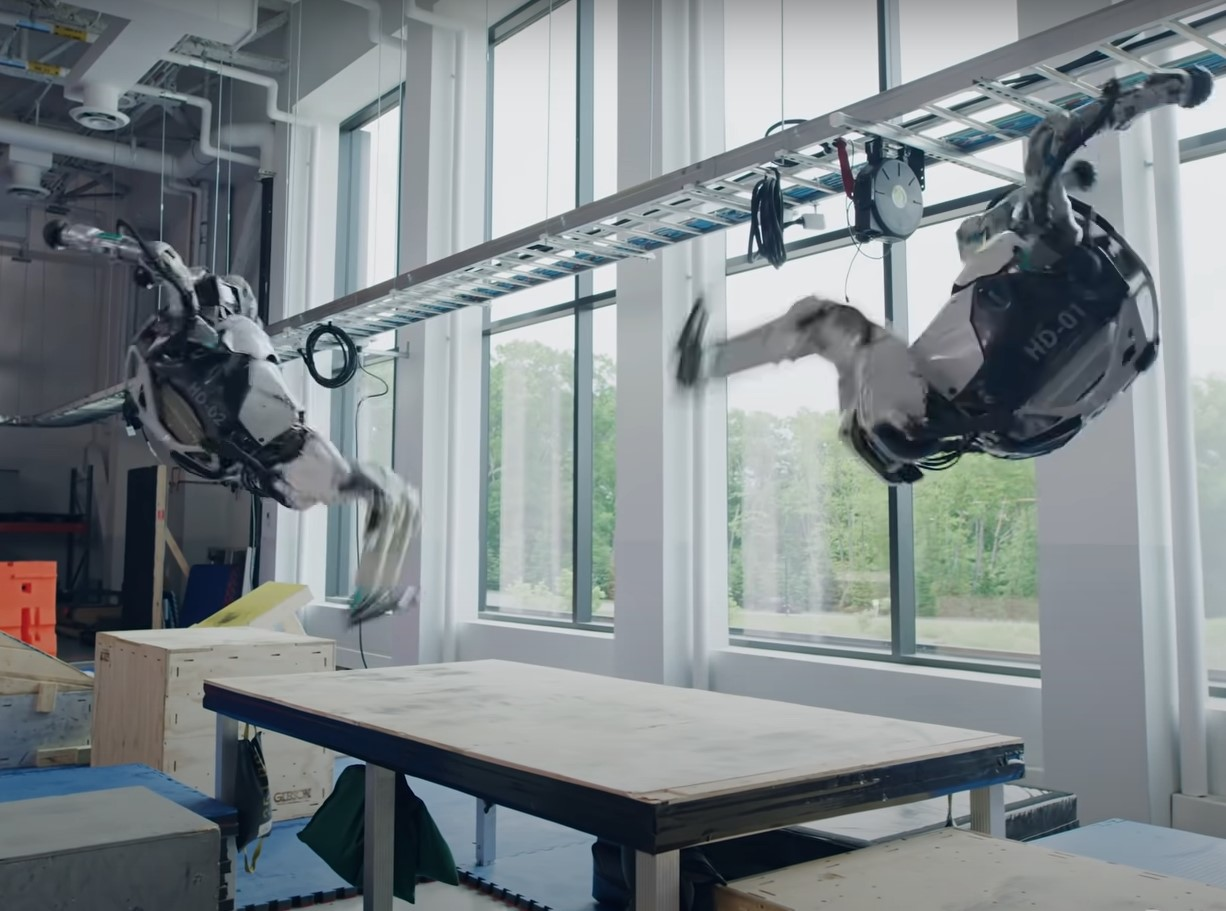
\includegraphics[height=.43\linewidth]{dance2.jpg}
    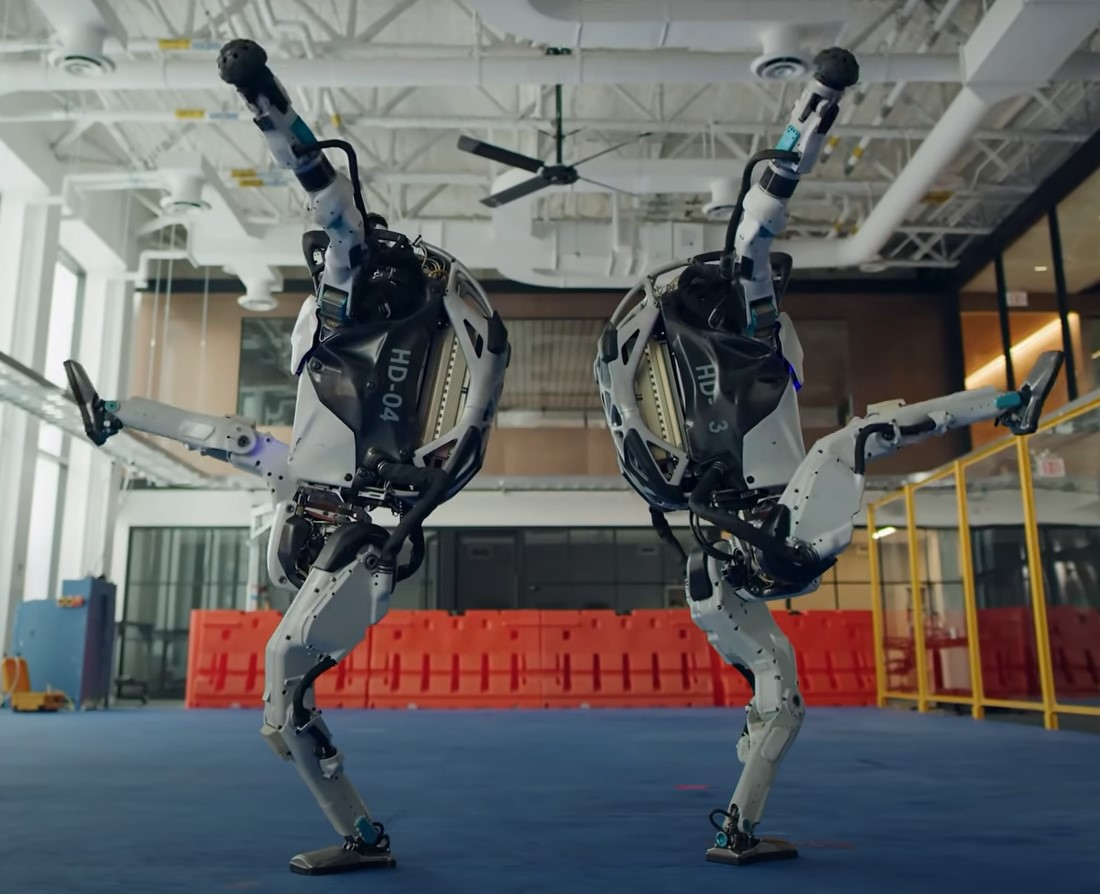
\includegraphics[height=.4\linewidth]{dance3.jpg}
    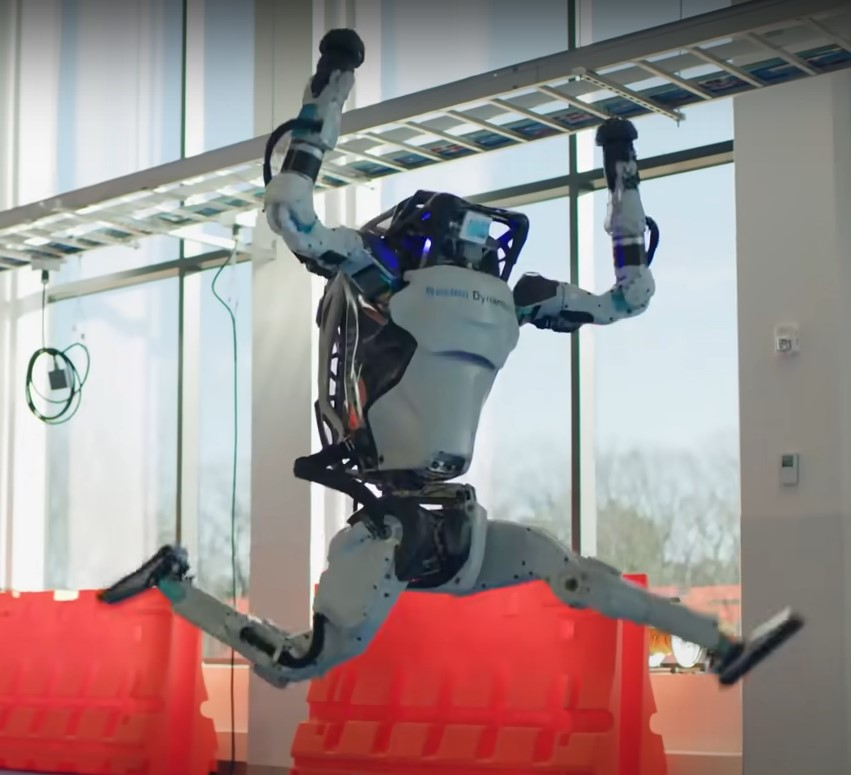
\includegraphics[height=.4\linewidth]{dance4.jpg}
    \caption{\label{fig:atlas_dance}Atlas机器人完成各种高难度动作}
\end{figure}

除Atlas外,美国的其他研究机构也在仿人机器人领域取得了瞩目的成就。密歇根大学的Jessy Grizzle教授在1997年开始研究平面仿人机器人,先后研发了RABBIT(\aref{subfig:RABBIT})
和MABEL(\aref{subfig:MABEL}),MABEL利用弹性机构储能,大大突破了电机功率密度的限制,可在平面约束下以1.95m/s进行奔跑,并且能够跨越障碍。在此基础上,Grizzle又和
俄勒冈州立大学的Jonathan Hurst教授合作研发了ATRIAS\cite{rezazadeh2015toward}(\aref{subfig:ATRIAS})以及MARLO\cite{buss2014preliminary}(\aref{subfig:MARLO})
两代3D仿人机器人,设计有板簧储能元件以及轻量化的腿部连杆,几乎所有的质量都集中在身体部位,能以最高9.1km/h的速度奔跑,并能应对台阶、室外斜坡等复杂路况。

\begin{figure}[htbp]
    \centering
    \subcaptionbox{RABBIT\label{subfig:RABBIT}}
        {%
            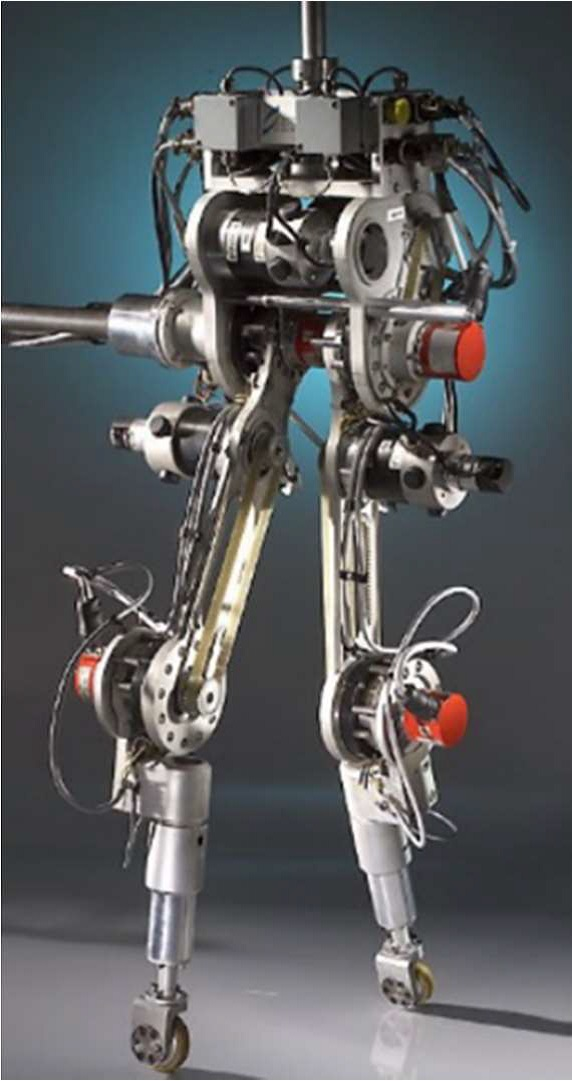
\includegraphics[height = .225\textheight]{michigan1.jpg}}
    \hspace{1in}
    \subcaptionbox{MABEL\label{subfig:MABEL}}
        {%
            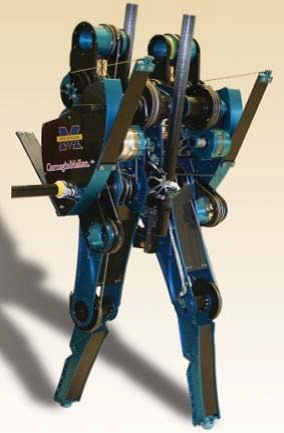
\includegraphics[height = .225\textheight]{michigan2.png}}

    \subcaptionbox{ATRIAS\label{subfig:ATRIAS}}
        {%
            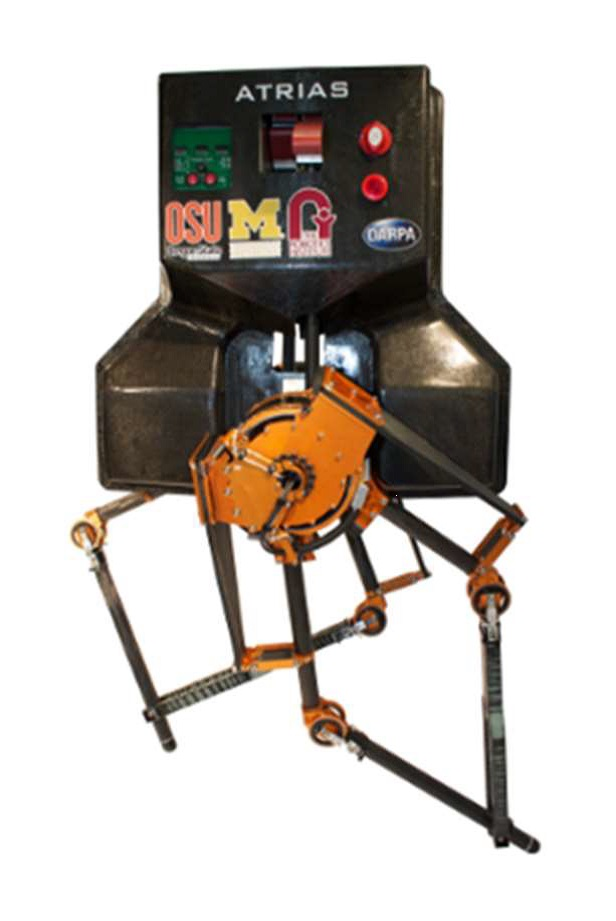
\includegraphics[height = .225\textheight]{michigan3.jpg}}
    \hspace{1in}
    \subcaptionbox{MARLO\label{subfig:MARLO}}
        {%
            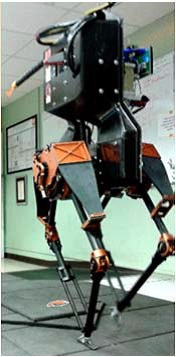
\includegraphics[height = .225\textheight]{michigan4.jpg}}
    \caption{Jessy Grizzle和Jonathan Hurst合作研发的仿人机器人\label{fig:michigan_biped}}
\end{figure}

Jonathan Hurst在此前研究的基础上创办了Agility Robotics,而后者于2017年发布了仿人机器人Cassie\cite{Cassie}(\aref{subfig:Cassie})。Cassie由电机驱动,每条腿具备5个驱动自由度和
2个欠驱动自由度,能以2.1m/s的速度高速行走,并具备对户外复杂地形的良好适应能力。2019年Agility Robotics又发布了给cassie加入上身和双臂的仿人机器人Digit\cite{Digit}(\aref{subfig:Digit}),
Digit的设计目标在于和无人驾驶车队配合,解决无人配送最后的送货上门问题。

\begin{figure}[htbp]
    \centering
    \subcaptionbox{Cassie\label{subfig:Cassie}}
        {%
            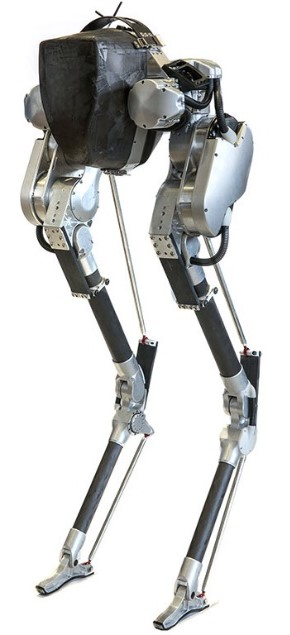
\includegraphics[height = .4\linewidth]{cassie.jpg}}
    \hspace{1in}            
    \subcaptionbox{Digit\label{subfig:Digit}}
        {%
            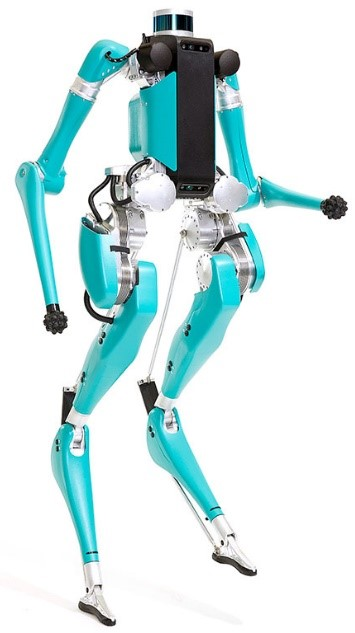
\includegraphics[height = .4\linewidth]{digit.jpg}}
    \caption{Agility Robotics研发的两款仿人机器人产品\label{fig:michigan_biped}}
\end{figure}

\subsection{其他国家仿人机器人研究现状}

德国慕尼黑工业大学在2009年发布了仿人机器人Lola\cite{buschmann2009humanoid}。Lola多个关节采用了电机+滚珠丝杆的传动方式,尽可能减小腿部的转动惯量,可以以2.4km/h的速度步行。在2021年最新发布的视频中,
Lola以及可以应对不规则的路面,并可以在走过易打滑路面的时候利用双手支撑侧面墙壁以避免失稳\cite{Lola}(\aref{fig:lola})。

\begin{figure}[htbp]
    \centering
    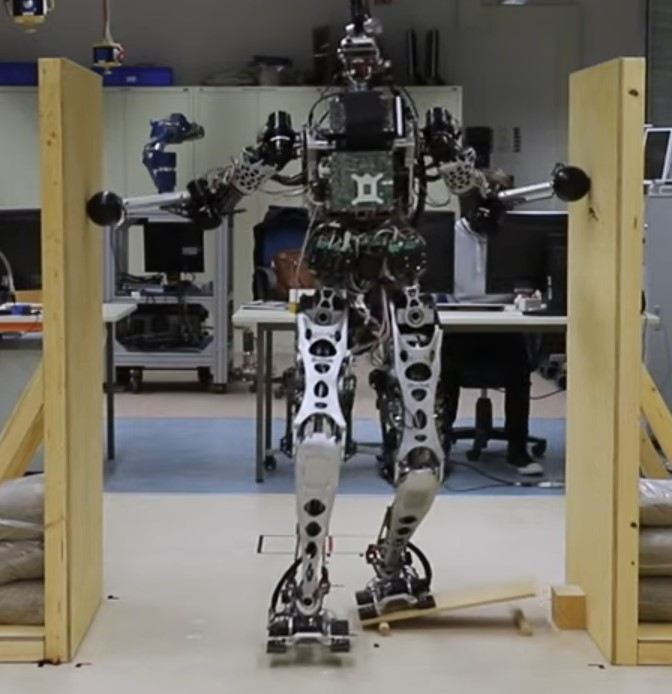
\includegraphics[width=0.60\textwidth]{lola.jpg}
    \caption{\label{fig:lola}慕尼黑工大Lola机器人手臂辅助行走}
\end{figure}

意大利技术研究院(Italian Institute of Technology,简称IIT)在腿足机器人领域有着许多卓越的成果,2007年IIT推出了儿童尺寸的仿人机器人iCub\cite{tsagarakis2007icub}(\aref{subfig:iCub}),iCub装备了
具有触觉感知的人造皮肤等一系列传感器,但行走并不是它的主要设计目标,因此iCub的运动能力很差。除了iCub外,IIT在2012年公布了以行走功能为重点的COMAN\cite{dallali2012global}(\aref{subfig:COMAN}),
它的关节由SEA驱动,SEA带来的关节力控制效果使得COMAN在站立平衡恢复方面展现出优异的性能,但电机的功率限制决定了COMAN的行走性能非常一般。之后2013年IIT又参与了欧盟的
Whole-body Adaptive Locomotion and Manipulation项目,在随后的四年中研发了两款WALK-MAN机器人\cite{tsagarakis2017walk}(\aref{subfig:WALK-MAN}),但运动性能相比COMAN并未有显著的提升。

\begin{figure}[htbp]
    \centering
    \subcaptionbox{iCub\label{subfig:iCub}}
        {%
            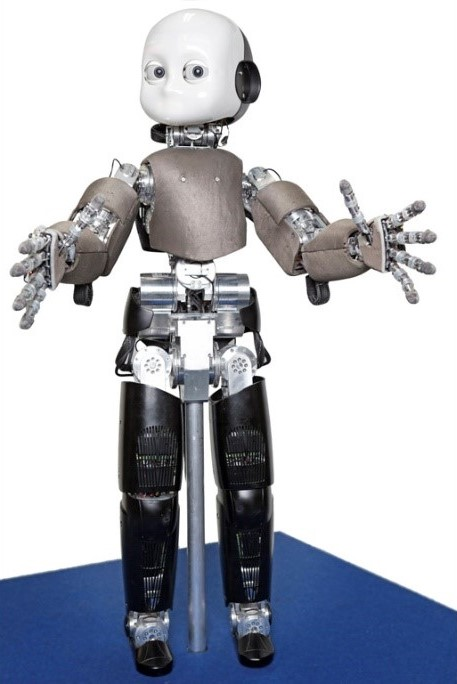
\includegraphics[height = .4\linewidth]{iCub.jpg}}
    \subcaptionbox{COMAN\label{subfig:COMAN}}
        {%
            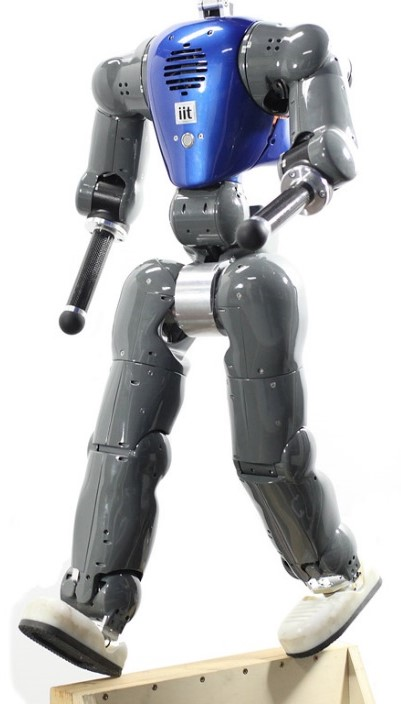
\includegraphics[height = .4\linewidth]{coman.jpg}}
    \subcaptionbox{WALK-MAN\label{subfig:WALK-MAN}}
        {%
            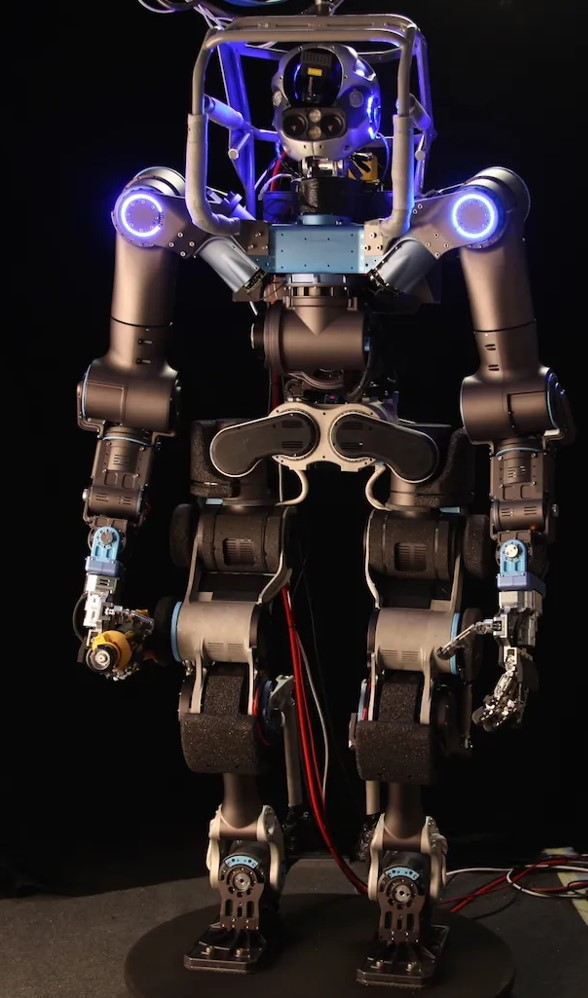
\includegraphics[height = .4\linewidth]{walkman.jpg}}            
    \caption{Agility Robotics研发的两款仿人机器人产品\label{fig:iit_biped}}
\end{figure}

韩国先进技术研究院(Korea Advanced Institute of Science and Technology,简称KAIST)从2002年开始迭代研发了一系列KHR/HUBO仿人机器人,从2002年的KHR-1开始,
到2013年参加DRC的DRC-HUBO已经是第七代了。DRC-HUBO采用轮腿混合的设计,既能以仿人形态行走,也能跪下利用膝盖上的轮子移动\cite{zucker2015general}(\aref{fig:kaist_hubo})。
可以根据不同情境选择移动方式的优势使得DRC-HUBO最终夺得了DRC2015的冠军。

\begin{figure}[htbp]
    \centering
    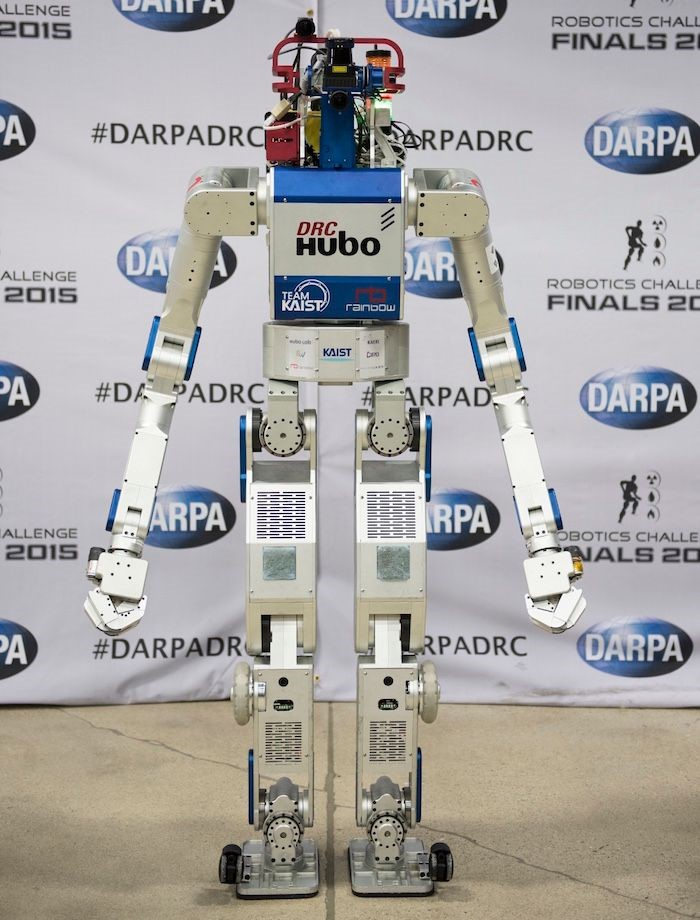
\includegraphics[height=.4\linewidth]{kaist1.jpg}
    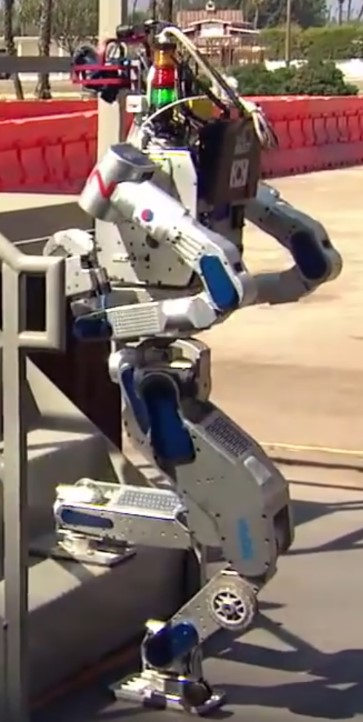
\includegraphics[height=.4\linewidth]{kaist2.jpg}
    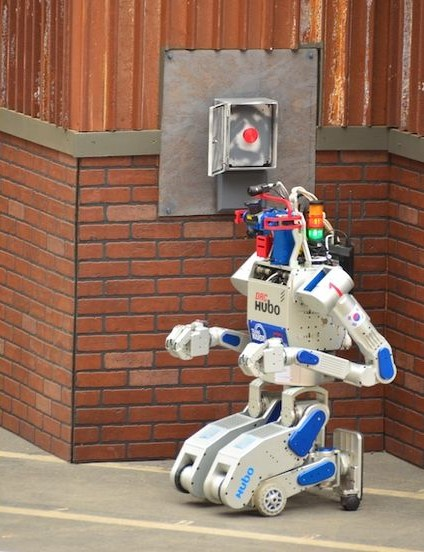
\includegraphics[height=.4\linewidth]{kaist3.jpg}
    \caption{\label{fig:kaist_hubo}KAIST-HUBO机器人及其多种运动形态}
\end{figure}

\subsection{我国仿人机器人研究现状}
早在1985年哈尔滨工业大学就研制了HIT-III仿人机器人,这也被认为是我国最早的仿人机器人\cite{谢涛2002}。该机器人由电机驱动,仅仅能够进行基本的静态步行。
国防科技大学1995年公布的KDW-III仿人机器人也仅能实现0.36km/h的静态步行。随后国防科技大学又在2001年公布了仿人机器人“先行者”(\aref{subfig:poineer}),是国内第一台具有可运动四肢的仿人机器人。
北京理工大学2000年开始了仿人机器人的研究,之后发布了“汇童”系列仿人机器人(\aref{subfig:sboy})。2006年发布的第二代汇童机器人已经具备了1km/h的动态行走能力,同时可以实现打太极、舞剑等全身动作。
第四代和第五代又分别实现了表情控制和打乒乓球的功能。目前最新的第六代汇童机器人可以实现倒地爬起、原地跳跃等功能\cite{huang2019historical}。浙江大学于2011年公布了仿人机器人KONG-II\cite{sun2011balance}(\aref{subfig:KONG})。
该机器人全身共计32个自由度,高160cm,重65kg,步行速度可达1.07km/h,能够实现和人对打乒乓球的功能。

\begin{figure}[htbp]
    \centering
    \subcaptionbox{先行者\label{subfig:poineer}}
        {%
            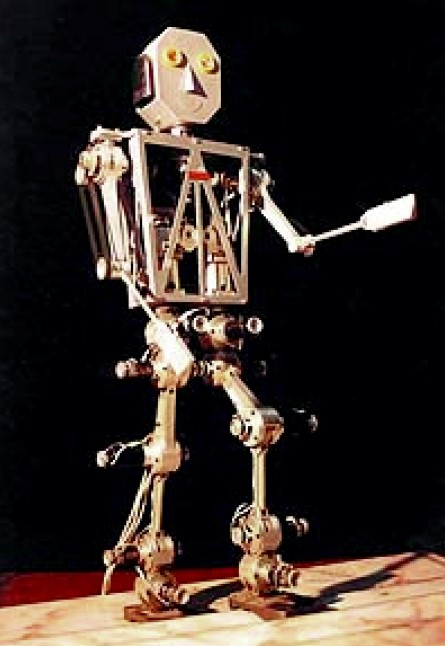
\includegraphics[height = .4\linewidth]{domestic1.jpg}}
    \subcaptionbox{汇童\label{subfig:sboy}}
        {%
            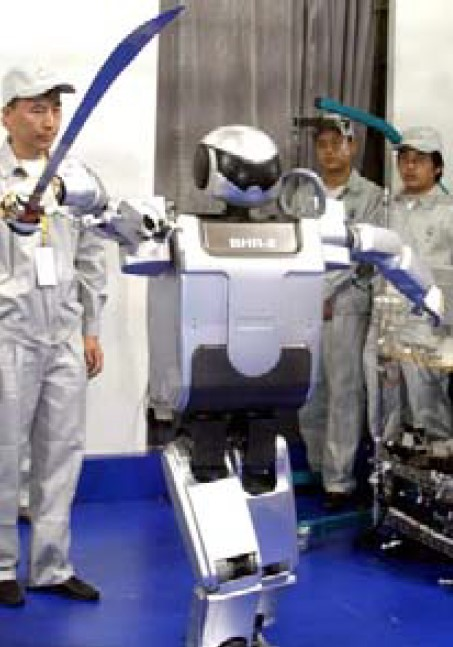
\includegraphics[height = .4\linewidth]{domestic2.jpg}}
    \subcaptionbox{KONG\label{subfig:KONG}}
        {%
            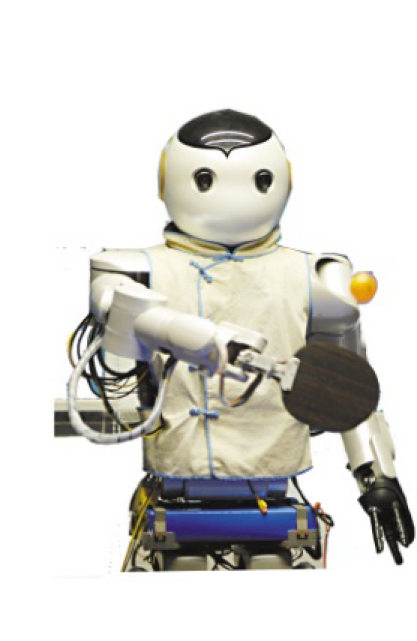
\includegraphics[height = .4\linewidth]{domestic4.png}}              
    % \subcaptionbox{THBIP-I\label{subfig:THBIP-I}}
    %     {%
    %         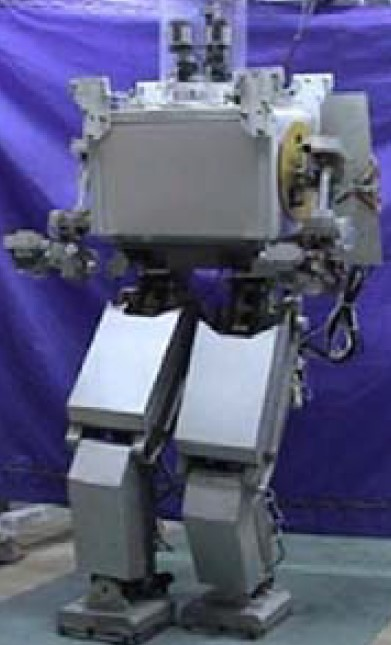
\includegraphics[height = .4\linewidth]{domestic3.jpg}}         
    \caption{国内部分仿人机器人\label{fig:domes_biped}}
\end{figure}

截至2022年,国内公开的仿人机器人中,更多还是借鉴了日本在仿人机器人领域的技术路线,采用高速电机加大速比减速器的关节驱动方案,运动性能基本还都局限在低速静态步行,
难以实现仿人机器人的动态步行,相较国外还有相当大的差距。
\section{腿足运动控制最新进展}
腿的作用在于,机器人能用腿上的末端执行器来推“地”从而为身体提供主动避震,
使得机器人身体的运动要比地表的轮廓更平滑。我们把所有用来推“地”的末端执行器统一叫做“足”,
不管它们的形式和功能具体是什么。腿可以暂时离开地面来迈步,因此可以通过不连续的地形,
在轮子无法到达的地方运动。无论腿的数量、运动学构型和自由度数,
足的类型(平面足,可变形足,点足,轮足)如何变化,根本的原理是一样的。
因此,最近几年原本在平面足人形机器人上发展的方法也快速适配了四足机器人以及其他形式足的腿足机器人。

控制的目标是找到足够多的可以在足和环境之间建立接触的位置,并且执行对应的动力学可行的轨迹。
为了处理腿足运动控制的关键难题——交替的触地和对应的接触力约束,
目前几乎推广到所有形式的腿足机器人的通用方法大量使用了数值轨迹优化及其在线实现——MPC。

除了将这种通用的方法适配到不同数量的腿和不同类型的足,
近几年在腿足运动控制领域的主要进展是如何用“提纯”的模型和“提纯”的数值模型来处理轨迹优化问题。
这使得从在多为平地的仿人行走到更多样的机器人形态
,更通用的不平整地形的多接触运动的转换成为可能。
除了将这种通用的方法适配到不同数量的腿和不同类型的足,
近几年在腿足运动控制领域的主要进展是如何用“提纯”的模型和“提纯”的数值模型来处理
轨迹优化问题。这使得从在多为平地的仿人行走到更多样的机器人形态
,更通用的不平整地形的多接触运动的转换成为可能。

\subsection{腿足运动控制的典型方法}
% The dynamics of legged locomotion: 
牛顿方程说明和环境接触产生的外力$\boldsymbol{f}_i$减去重力$m\boldsymbol{g}$决定了机器人质心$\boldsymbol{c}$变化的方向:
\begin{equation}
    \label{equ:newton}
    m(\ddot{\boldsymbol{c}}-\boldsymbol{g})=\sum_i \boldsymbol{f}_i
\end{equation}
其中$m$是机器人的总质量。同时对应的欧拉方程表明接触点$s_i$相对质心$c$的位置是控制机器人身体相对质心的角动量$L$的关键:
\begin{equation}
    \label{equ:euler}
    \dot{\boldsymbol{L}}=\sum_i\left(\boldsymbol{s}_i-\boldsymbol{c}\right) \times \boldsymbol{f}_i
\end{equation}

% Artificial synergy synthesis 
基于质心动力学的方法认为,应该更加关注和地面接触力直接绑定的质心动力学
\aref{equ:newton}和\aref{equ:euler},
而不是和关节力矩更直接绑定的机器人的精准关节姿态\cite{vukobratovic1972contribution},如\aref{fig:centroid}所示。
\begin{figure}[htbp]
    \centering
    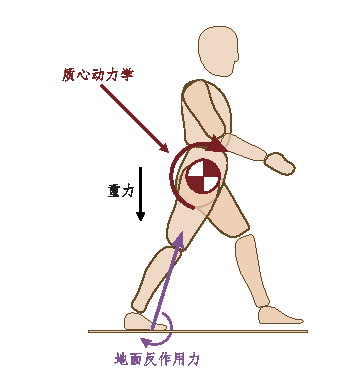
\includegraphics[width=.5\linewidth]{质心动力学.eps}
    \caption{\label{fig:centroid}质心动力学及其与全身动力学的联系释图(图源~\cite{carpentier2016center})}
\end{figure}
这种方法在现在是机器人运动控制的核心,但在需要紧密协调机器人平衡和姿态的情况下,基于完整多刚体拉格朗日动力学的方法才是首选,
因为它天然包含了质心动力学\cite{orin2013centroidal}。

腿足运控的难题之一是接触力通常是单边的:机器人只能推接触表面,而不能拉。因此接触力$f_i$只能朝向特定的方向,由摩擦锥来约束。
另外,每个接触都是二元的:要么有接触和接触力,要么没有接触也没有接触力。当腿和某个面碰撞,也会产生冲击力。
触地转换和冲击是影响连续动力学\aref{equ:newton}和\aref{equ:euler}的离散事件,从这个角度讲腿足机器人的动力学是混合的,
这是难题之二。

理论上,从机器人可以执行合适的接触力来避免摔倒的状态中,我们可以定义可行状态(viable states)。周期运动(周期踏步?)和平衡点
显然是可行的,并且如果机器人能从给定状态在几步内达到这样一个循环或者是平衡点,那这样的状态也是可行的\cite{wieber2002stability}。
这就是目前许多现有腿足运控方法的关键\cite{wieber2016modeling}——可捕获性分析\cite{pratt2006velocity}的要义。

接触点$s_i$的序列通常要考虑机器人所在环境及其目标点、运动学和静平衡约束\cite{escande2013planning},
用随机采样点的方法在时空域上预先规划好,这个过程称作落脚点规划。预规划好的落脚点在后续执行的过程中可以根据实际的地形
和外界扰动来调整cite{feng2016robust}。对应的质心运动和角动量可以通过在线MPC的框架来得到\cite{wieber2006trajectory},
该框架在考虑质心动力学\aref{equ:newton}和\aref{equ:euler}的同时需要保证机器人的状态始终是可捕获的\cite{wieber2016modeling}。

当机器人在平地上运动,所有接触点$s_i$都是共面的,接触力$f_i$通常会退化到他们的零力矩点(ZMP),而ZMP在接触点组成的凸包内\cite{wieber2002stability}
(通过单边接触约束的多面体投影,非平面的接触点也有类似的性质\cite{caron2016zmp})。在这种情况下,预先定义好质心在竖直方向上的运动可以得到高效的线性模型。
最常见的是线性倒立摆模型(LIP),它假设质心在平面内运动并且角动量为0\cite{kajita1991study}。考虑非零的角动量并不影响模型的线性,但很少有人这样做,
可能是在平地上行走时这样做的好处并不多\cite{koolen2012capturability}。

通常用逆运动学\cite{kajita2003resolved},或者笛卡尔空间下的全身动力学的反馈线性化\cite{wieber2000constrained},来让机器人的整个身体去执行
规划出的质心运动,角动量和触地位置,用二次规划(Quadratic Programs)来考虑瞬时的运动学、动力学、力和力矩约束\cite{wieber2000constrained, kuindersma2014efficiently}。
分层QP可以在控制目标函数中考虑不同的优先级\cite{escande2014hierarchical},但存在奇异的问题\cite{wieber2017geometric}。逆运动学和反馈线性化对模型误差尤其是位置误差,
以及对机器人平衡至关重要的地面接触的稳定性和刚度非常敏感。基于欠驱动(passivity)的方法更不依赖于准确的接触模型\cite{henze2016passivity, kurtz2020approximate},
是上述方法很有前景的一种替代。
\begin{figure}[htbp]
    \centering
    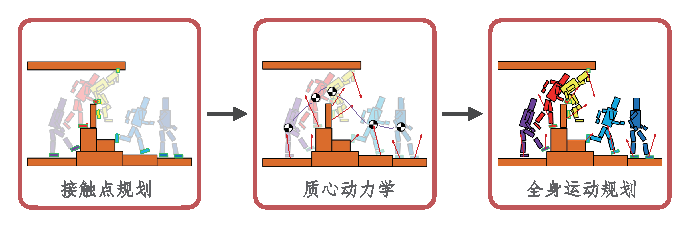
\includegraphics[width=1.0\linewidth]{仿人经典控制框架.eps}
    \caption{\label{fig:typical_control}典型的控制框架由主要由三阶段组成:接触规划,质心动力学级规划和全身控制
                (图源~\cite{carpentier2016center})}
\end{figure}
\aref{fig:typical_control}所示腿足运控的通用方法,原本是为仿人行走开发的,并且在Kawada的HRP-2\cite{takenaka2009real},
本田的Asimo\cite{takenaka2009real},Aldebaran的Nao\cite{gouaillier2010omni},波士顿动力的Atlas\cite{Kuindersma2020Recent}等等一系列的机器人上得到了成功的验证。
最近这种方法也被适配到了诸如ANYbotics的ANYmal\cite{bellicoso2018dynamic},IIT的HyQ\cite{mastalli2017trajectory},
MIT的Cheetah\cite{di2018dynamic}等四足机器人以及Aldebaran的pepper\cite{lafaye2014linear},ETHZ的ANYmal\cite{bjelonic2020rolling}
和Ascento\cite{klemm2020lqr}等轮足机器人上。

\section{本文的主要研究内容}
本文针对仿人机器人跑跳步态的实现,首先简要介绍仿人机器人的实验平台“悟空
-II”机器人,其次根据仿人机器人状态机设计,分别对机器人处于单腿支撑相时与双腿
腾空相时设计控制器,同时面对机器人在前进过程中前进方向出现偏差的问题,提出相
应的解决方法。

本文的主要研究内容:

1) 构造了仿人机器人跑跳步态的状态机,设计了姿态平衡控制器和高度控制器。
将仿人机器人前进过程分为单腿支撑相与双腿腾空相。机器人处于单腿支撑相
时,设计控制器保持身体的姿态;利用对地面反作用力的控制维持身体质心高
度,为机器人能够采用跑跳步态前进提供前提。

2) 设计了仿人机器人快速运动的速度控制器。描述结合运动学与陀螺仪数据,采
用卡尔曼滤波器估计质心速度的方法;重点介绍摆动腿的轨迹规划与落脚点控
制,根据LIP 模型控制,利用机器人摆动腿的落脚点实现对机器人的速度控制,
同时规划摆动腿摆动曲线以及添加摆动腿摆动过程中的重力补偿。

3) 设计了仿人机器人的转向运动控制。针对机器人前进过程中会出现方向偏差的
问题,采用对支撑腿髋关节偏航关节的运动规划实现机器人低速运动下的方向
控制;机器人高速前进时,采用利用腰关节转动平衡机器人支撑腿与摆动腿运
动产生的转动力矩;同时将仿人机器人的偏转力矩加入机器人的姿态控制器中,
期望实现仿人机器人的方向上的控制。

4) 在WuKong-IV仿人机器人实验平台上开展实验,验证上述控制算法。成功验证
身体姿态控制器与质心高度控制器的有效性;利用卡尔曼滤波器获得更加准确
的质心速度,利用落脚点控制实现WuKong-IV机器人前进速度的控制;改进机
器人前进过程中的方向控制。

\section{本文主要结构}
根据本文的研究内容以及顺序,各章节的内容安排如下:

第一章 本章主要介绍国内外仿人机器人的情况,对国内外知名仿人机器人简单介绍,
介绍仿人机器人跑跳步态的研究现状。

第二章 本章主要介绍WuKong-IV仿人机器人实验平台,简要描述实物平台的机械结
构与电气结构,根据实物模型构造简化连杆模型,规定世界坐标系与各连杆
坐标系的方向,本章介绍了仿人机器人的状态机描述,状态的循环稳定的切
换形成仿人机器人的跑跳步态,介绍仿人机器人处于单腿支撑下的控制方法,
实现仿人机器人身体姿态平衡与质心高度平衡。

第三章 本章利用卡尔曼滤波实现对机器人质心速度更准确的估计。介绍仿人机器人
的速度控制与摆动腿规划,利用摆动腿的落脚点的位置实现对于仿人机器人
前进速度的控制,规划一个步态周期的摆动腿曲线,为摆动腿的运动增加重
力补偿。

第四章 本章针对仿人机器人前进过程中方向偏转的问题,利用规划腰关节摆动实现
偏转力矩的平衡,同时将偏转考虑进仿人机器人的姿态控制,期望实现前进
方向的控制。

第五章 本章对本文工作进行简要总结,提出工作的不足之处,并对进一步的工作提
出一些展望。
\chapter{仿人机器人状态估计}
\section{机器人浮动基模型}
\begin{figure}[htbp]
    \centering
    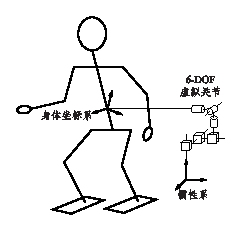
\includegraphics[width=.6\linewidth]{浮动基.eps}
    \caption{\label{fig:floating_base}仿人机器人浮动基运动模型}
\end{figure}

与工业机械臂、轮履式机器人等传统类型机器人的运动不同,仿人机器人或者说腿足机器人的运动包括两个显著的特征:
\begin{itemize}
    \item 机器人和环境之间不存在刚性的连接,或者说机器人的基座是“浮动”的。
    \item 机器人和环境的接触是不连续的,随着腿的交替运动,机器人的动力学也随之产生阶段性的不连续变化。
\end{itemize}

基于以上两个特征,浮动基描述成为了现在对腿足运动通用的表示方法。如\aref{fig:floating_base}所示,我们假设仿人机器人和环境之间存在$n_b$个虚拟关节,它们的数值组成了浮动基的坐标$\boldsymbol{q}_b$,
$\boldsymbol{q}_b$再加上机器人身上的$n_j$个驱动关节组成的坐标$\boldsymbol{q}_j$,组成了机器人的广义坐标$\boldsymbol{q}$,即:
\begin{equation}
    \label{equ:general_coor}
    \boldsymbol{q}=\left(\begin{array}{c}
        \boldsymbol{q}_b \\
        \boldsymbol{q}_j
        \end{array}\right)
\end{equation}
其中,
\begin{equation}
    \label{equ:floating_coor}
    \boldsymbol{q}_b=\left(\begin{array}{c}
        \boldsymbol{q}_{b_P} \\
        \boldsymbol{q}_{b_R}
        \end{array}\right) \in \mathbb{R}^3 \times SO(3)
\end{equation}
\aref{equ:floating_coor}中$ \boldsymbol{q}_{b_P}$表示浮动基的位置,$\boldsymbol{q}_{b_R}$表示浮动基的姿态。在本文中我们用笛卡尔坐标表示位置,$rpy$姿态角表示姿态,因此$n_b = 6$。

基于这样的坐标表示,如何利用机器人的本体感知,即惯性测量单元(Inertial Measurement Unit,IMU)和机器人内部关节的编码器,来获得机器人的浮动基坐标,对于实现机器人的稳定运动控制来说是至关重要的。

本章介绍了利用卡尔曼滤波的方法来实现浮动基坐标的估计,标准卡尔曼滤波的迭代过程可由\aref{alg:KF}表示。\aref{sec:contact_est}和\aref{sec:com_est}分别介绍了对机器人与环境的接触状态和机器人浮动基相对于惯性系的
位置、速度的估计方法。
\begin{algorithm}[htbp] 
\setstretch{1.3}
\caption{线性卡尔曼滤波} 
\label{alg:KF} 
\begin{algorithmic}[1] %这个1 表示从第一行开始显示行号,不写就不会显示行号
\STATE{\fangsong{\textbf{输入}}:$\hat{\boldsymbol{x}}_{k-1}, \tilde{\boldsymbol{z}}_k, \boldsymbol{\Sigma}_{k-1}, \boldsymbol{Q}_{w_k}, \boldsymbol{R}_{v_k}$}
\STATE{\fangsong{\textbf{输出}}:$\hat{\boldsymbol{x}}_{k}, \tilde{\boldsymbol{z}}_k, \boldsymbol{\Sigma}_{k}$}
\STATE{\textbf{Step 1}\ \fangsong{初始化}$\boldsymbol{A}_0$,$\boldsymbol{B}_0$,$\boldsymbol{H}_0$}
\STATE{\textbf{Step 2}\ \fangsong{预测}:}
\STATE{$\ \ \ \ \ \ \ \ \begin{gathered}
        \hat{\boldsymbol{x}}_{k \mid k-1}=\boldsymbol{A}_k \hat{\boldsymbol{x}}_{k-1}+\boldsymbol{B}_k \boldsymbol{u}_k \\
        \boldsymbol{\Sigma}_{k \mid k-1}=\boldsymbol{A}_k \boldsymbol{\Sigma}_{k-1} \boldsymbol{A}_k^T+\boldsymbol{Q}_{w_k}
        \end{gathered}$}
\STATE{\textbf{Step 3}\ \fangsong{计算卡尔曼增益}:}
\STATE{$\ \ \ \ \ \ \ \ \boldsymbol{K}_k=\boldsymbol{\Sigma}_{k \mid k-1} \boldsymbol{H}_k^T\left(\boldsymbol{H}_k \boldsymbol{\Sigma}_{k \mid k-1} \boldsymbol{H}_k^T+\boldsymbol{R}_{v_k}\right)$}
\STATE{\textbf{Step 4}\ \fangsong{校正}:}
\STATE{$\ \ \ \ \ \ \ \ \begin{gathered}
    \hat{\boldsymbol{x}}_{k \mid k}=\hat{\boldsymbol{x}}_{k \mid k-1}+\boldsymbol{K}_k\left(\tilde{\boldsymbol{z}}_k-\boldsymbol{H}_k \hat{\boldsymbol{x}}_{k \mid k-1}\right) \\
    \boldsymbol{\Sigma}_{k \mid k}=\left(\mathbf{I}-\boldsymbol{K}_k \boldsymbol{H}_k\right) \boldsymbol{\Sigma}_{k \mid k-1}
    \end{gathered}$}

\end{algorithmic}
\end{algorithm}
\section{触地状态估计}
\label{sec:contact_est}
\subsection{概率触地模合}
实际上,我们不能完全信任控制器会按时将脚抬离或者放回地面,完美地按照规划出的相位执行。同样地,我们也不能假设地面是完全平整的,
由于复杂的地形或者是未知的物体,地面的高度可能是未知的。在没有外部力传感器的情况下,我们必须从关节编码器的数据,本体力感知,
以及腿的动力学模型来估计外部作用力。编码器有离散误差,同时模型误差会导致在没有外力的时候也会计算出非0的外力。
这些单一的测量没有一个能告诉我们腿的真实状态,但我们能从每个测量中获取信息,并且用这些信息来得到某条腿是否有可能和地面接触的一个
更好的估计$\hat s$,$\hat s \in \left\{0=swing, 1=contact\right\}$。完美的触地检测算法满足$\hat s = s$,$s$表示触地状态的真值。
由于要使用多种测量,使用卡尔曼滤波器来实现数据融合是很自然的。将脚和地面接触的整体估计概率作为卡尔曼滤波器的状态,即:
\begin{equation}
    \label{equ:est_state}
    \hat{\boldsymbol{x}}_k=\left\{\begin{array}{c}
        P_l(c) \\
        P_r(c)
        \end{array}\right\}_k
\end{equation}
自然而然地,我们可以用概率接触模型作为先验来融合所有可用的数据。虽然测量中涉及到的动力学很复杂,但把接触的概率作为状态,
我们就能用一个简单的线性卡尔曼滤波来实现。在估计时使用概率而不是离散的二进制接触状态的好处之一是,在概率增大或者减小时
我们可以预测会发生接触状态的变化。
\subsection{预测——过程模型}

对于给定的步态规划和当前某条腿的相位$\phi$,步态规划器会给出每条腿期望的接触状态$s_{\phi}$。在理想情况下,$s = s_{\phi}$,
并且状态切换是同时发生的。然而机器人的控制系统很容易有延时,这可能导致腿抬得晚了,或者由于摆动腿轨迹跟随的误差以及未知的地面高度变化
导致触地触地提前或者晚了。

为了解决这些问题,我们可以建立一个概率模型,来在给定腿的规划接触状态和在支撑相 或者摆动相 的子相的情况下得到触地的期望值。
对于给定接触状态和子相百分比,触地概率有如下形式:
\begin{equation}
    \label{equ:est_contact_prob}
    \begin{aligned}
        P\left(c \mid s_\phi, \phi\right)= & \frac{1}{2}\left(s_\phi\left[\operatorname{erf}\left(\frac{\phi-\mu_{c_0}}{\sigma_{c_0} \sqrt{2}}\right)+\operatorname{erf}\left(\frac{\mu_{c_1}-\phi}{\sigma_{c_1} \sqrt{2}}\right)\right]+\right. \\
        & \left.\bar{s}_\phi\left[2+\operatorname{erf}\left(\frac{\mu_{\bar{c}_0}-\phi}{\sigma_{\bar{c}_0} \sqrt{2}}\right)+\operatorname{erf}\left(\frac{\phi-\mu_{\bar{c}_1}}{\sigma_{\bar{c}_1} \sqrt{2}}\right)\right]\right)
        \end{aligned}
\end{equation}
其中$s_{\phi}$表示支撑相或者摆动相之间的切换,均值$\mu$表示接触状态切换的期望子相值,方差$\sigma^2$由触地相的子相值的可变性(variability)决定。
\begin{figure}[htbp]
    \centering
    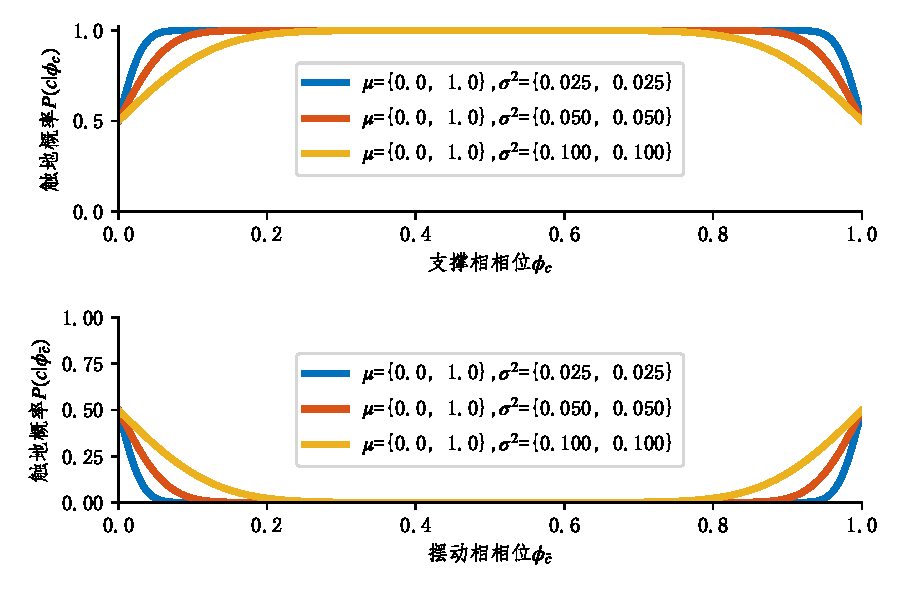
\includegraphics[width=.75\linewidth]{gauss_phase.pdf}
    \caption{\label{fig:gauss_phase}基于相位的触地概率。对于预定状态和状态子相的完成进度,多个参数会定义触地的概率。}
\end{figure}
\aref{fig:gauss_phase}展示了基于相位和规划状态的不同方差的接触概率的两条曲线。
在触地相即将要开始和结束的阶段,腿出于触地状态的可能性是更小的,
而在摆动相的开始和结束阶段腿处于触底状态的可能性是更大的。因此这种模型可以被用作系统的瞬时输入,将各条腿叠在一起,
用每条腿的规划状态和相位,将其写成:
\begin{equation}
    \label{equ:est_input}
    \boldsymbol{u}_k=\left\{\begin{array}{c}
        P_l\left(c \mid s_\phi, \phi\right) \\
        P_r\left(c \mid s_\phi, \phi\right)
        \end{array}\right\}_k
\end{equation}
下面的协方差矩阵 大致表示了我们对基于相位的状态切换模型的置信度:
\begin{equation}
    \label{equ:est_process_noise}
    \boldsymbol{Q}_{w_k}=\left[\begin{array}{ccc}
        \sigma_{\phi, 1}^2 & \cdots & 0 \\
        \vdots & \ddots & \vdots \\
        0 & \cdots & \sigma_{\phi, N}^2
        \end{array}\right]_k
\end{equation}
由于我们只是通过融合当前可用的测量来看瞬时的接触检测,所以状态和输入矩阵可以定义为:
\begin{equation}
    \label{equ:est_process_matrix}
    \boldsymbol{A}_k=\mathbf{0}_N \quad \text { and } \quad \boldsymbol{B}_k=\mathbf{I}_N
\end{equation}
\subsection{校正——测量模型}

1)地面高度测量模型:在缺少环境感知系统的情况下,地面高度$z_g$可以概率地被建模出来。
表示地面高度的随机变量$z_g$符合高斯分布,即$Z_g \sim \mathcal{N}\left(\mu_{z_g}, \sigma_{z_g}^2\right)$。$\mu_{z_g}$表示地面高度的均值,
在没有外部信息时被设为0,因为我们无法对地形做出任何假设。类似地,方差大致和地形的“粗糙”程度对应。这样我们就能用地面高度的模型来根据当前机器人
足端在竖直方向的位置$p_z$得到触地的概率:
\begin{equation}
    \label{equ:est_height_prob}
    P\left(c \mid p_z\right)=\frac{1}{2}\left[1+\operatorname{erf}\left(\frac{\mu_{z_g}-p_z}{\sigma_{z_g} \sqrt{2}}\right)\right]
\end{equation}
\begin{figure}[htbp]
    \centering
    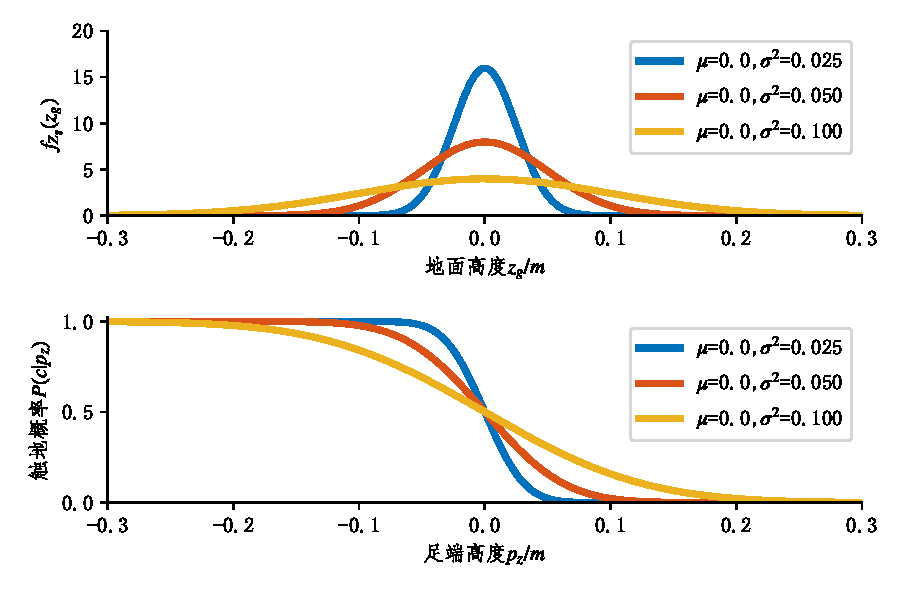
\includegraphics[width=.75\linewidth]{gauss_height.pdf}
    \caption{\label{fig:gauss_height}足底高度-触地概率图。高斯分布表示的地面高度${{z}_{g}}$,以及足底高度测量对应的触地概率。}
\end{figure}
\aref{fig:gauss_height}展示了地面的高斯模型,以及给定足端高度对应推理出的触地概率。每个图都有不同的参数对应不同地面粗糙度的估计。
最终$\mu_{z_g}$和$\sigma_{z_g}^2$的值可以从其他传感器信息或者之前的行走数据中获得。这个模型提供了第一次测量校正,
并且对应的协方差矩阵可以写为:
\begin{equation}
    \label{equ:est_height_noise}
    \tilde{\boldsymbol{z}}_{1, k}=\left\{\begin{array}{c}
        P_l\left(c \mid p_z\right) \\
        P_r\left(c \mid p_z\right)
        \end{array}\right\}_k \boldsymbol{R}_{v_{1, k}}=\left[\begin{array}{ccc}
        \sigma_{p_{z, l}}^2 & & 0 \\
        0 & & \sigma_{p_{z, r}}^2
        \end{array}\right]_k
\end{equation}
该协方差矩阵表示我们对接触高度模型信任度的度量。

2)接触力测量模型:足底的外力是唯一真实能表明发生了触地的信息。然而机器人当前并没有安装直接力传感器。通过第三部分中估计出的外力,
我们可以建立另一个力接触的简单概率模型,用随机变量$f_c$表示,$f_c$满足高斯分布:$F_c \sim \mathcal{N}\left(\mu_{f_c}, \sigma_{f_c}^2\right)$。
这里$\mu_{f_c}$是在接触处感知到的外力的均值,$\sigma_{f_c}^2$度量估计出的外力的噪声大小。对于给定估计接触力,触地概率可以写成:
\begin{equation}
    \label{equ:est_force_prob}
    P\left(c \mid f_z\right)=\frac{1}{2}\left[1+\operatorname{erf}\left(\frac{f_z-\mu_{f_c}}{\sigma_{f_c} \sqrt{2}}\right)\right]
\end{equation}
\begin{figure}[htbp]
    \centering
    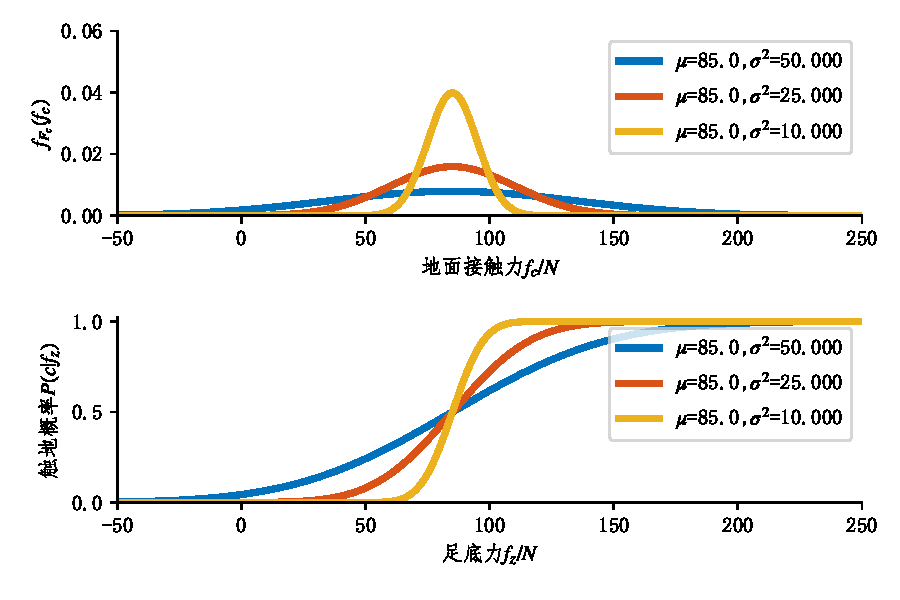
\includegraphics[width=.75\linewidth]{gauss_force.pdf}
    \caption{\label{fig:gauss_force}足底力-触地概率图。高斯分布表示的接触过程中的外力,以及足底外力测量对应的触地概率。}
\end{figure}
\aref{fig:gauss_force}展示了法向接触力和对应触地概率的关系,这个基于外力的概率是我们的第二个测量:
\begin{equation}
    \label{equ:est_force_noise}
    \tilde{\boldsymbol{z}}_{2, k}=\left\{\begin{array}{c}
        P_l\left(c \mid f_z\right) \\
        P_r\left(c \mid f_z\right)
        \end{array}\right\}_k \boldsymbol{\Sigma}_{v_{2, k}}=\left[\begin{array}{ccc}
        \sigma_{f_{z, l}}^2 & & 0 \\
        0 & & \sigma_{f_{z, r}}^2
        \end{array}\right]_k
\end{equation}

这两组单独的测量叠在一起组成了卡尔曼滤膜中的测量向量。类似地,每个测量的协方差矩阵组成了如下的块对角协方差矩阵:
\begin{equation}
    \label{equ:est_h_and_f}
    \tilde{\boldsymbol{z}}_k=\left[\begin{array}{c}
        \tilde{\boldsymbol{z}}_{1, k} \\
        \tilde{\boldsymbol{z}}_{2, k}
        \end{array}\right] \quad \boldsymbol{R}_{v_k}=\left[\begin{array}{cc}
        \boldsymbol{R}_{v_{1, k}} & \mathbf{0}_N \\
        \mathbf{0}_N & \boldsymbol{R}_{v_{2, k}}
        \end{array}\right]
\end{equation}
输出矩阵$\boldsymbol{H}_k$由两个$N\times N$的单位矩阵叠在一起组成:
\begin{equation}
    \label{equ:output_matrix}
    \boldsymbol{H}_k=\left[\begin{array}{l}
        \mathbf{I}_N \\
        \mathbf{I}_N
        \end{array}\right]
\end{equation}
其中$N$是足的个数,对于本文中的仿人机器人而言$N=2$。通过将步态规划器的期望接触状态和测量概率模型的结果融合,我们可以得到每条腿的实际接触状态的一个更好的估计。
由于我们把卡尔曼滤波器的$\boldsymbol{A}_k$设为$\mathbf{0}_N$,融合的过程也能通过贝叶斯定理下的静态最大似然方法来得到。
但我们还是用了标准的卡尔曼滤波来迭代更新(但这个过程是预先嵌入在标准卡尔曼滤波更新中的),这在机器人学中是更容易获得的。
\begin{algorithm}[htp]
\setstretch{1.3}
\caption{触地状态估计迭代过程} 
\label{alg:Framwork} 
\begin{algorithmic}[1] %这个1 表示从第一行开始显示行号,不写就不会显示行号
\STATE{\fangsong{\textbf{输入}}:$\hat{\boldsymbol{x}}_{k-1}, \tilde{\boldsymbol{z}}_k, \boldsymbol{\Sigma}_{k-1}, \boldsymbol{Q}_{w_k}, \boldsymbol{R}_{v_k}$}
\STATE{\fangsong{\textbf{输出}}:$\hat{\boldsymbol{x}}_{k}, \tilde{\boldsymbol{z}}_k, \boldsymbol{\Sigma}_{k}$}
\STATE{\textbf{Step 1}\ \fangsong{初始化}$\boldsymbol{A}_0, \boldsymbol{B}_0, \boldsymbol{H}_0, \boldsymbol{Q}_0,\boldsymbol{R}_0, \boldsymbol{\Sigma}_0,\boldsymbol{x}_0=\left[P_{l,0}(c), P_{r,0}(c)\right]^{\top}$}
\STATE{\textbf{Step 2}\ \fangsong{预测}:}
\STATE{$\ \ \begin{gathered}
        \hat{\boldsymbol{x}}_{k \mid k-1}=\boldsymbol{u}_k \\
        \boldsymbol{\Sigma}_{k \mid k-1}=\boldsymbol{Q}_{w_k}
        \end{gathered}$}
\STATE{\textbf{Step 3}\ \fangsong{计算卡尔曼增益}:}
\STATE{$\ \ \boldsymbol{K}_{k,1}=\boldsymbol{\Sigma}_{k \mid k-1} \left(\boldsymbol{\Sigma}_{k \mid k-1}+\boldsymbol{R}_{v_{1,k}}\right)$}
\STATE{$\ \ \boldsymbol{K}_{k,2}=\boldsymbol{\Sigma}_{k \mid k-1} \left(\boldsymbol{\Sigma}_{k \mid k-1}+\boldsymbol{R}_{v_{2,k}}\right)$}
\STATE{\textbf{Step 4}\ \fangsong{高度测量校正}:}
\STATE{$\ \ \begin{aligned}
    \hat{\boldsymbol{x}}_{k \mid k}&=\hat{\boldsymbol{x}}_{k \mid k-1}+\boldsymbol{K}_{k,1}\left(\tilde{\boldsymbol{z}}_{1,k}-\hat{\boldsymbol{x}}_{k \mid k-1}\right) \\
    \boldsymbol{\Sigma}_{k \mid {k,1}}&=\left(\mathbf{I}-\boldsymbol{K}_{k,1} \right) \boldsymbol{\Sigma}_{k \mid k-1}
    \end{aligned}$}
\STATE{\textbf{Step 4}\ \fangsong{接触力测量校正}:}
\STATE{$\ \ \begin{aligned}
    \hat{\boldsymbol{x}}_{k \mid k}&=\hat{\boldsymbol{x}}_{k \mid k-1}+\boldsymbol{K}_k\left(\tilde{\boldsymbol{z}}_{2,k}-\hat{\boldsymbol{x}}_{k \mid k-1}\right) \\
    \boldsymbol{\Sigma}_{k \mid {k,2}}&=\left(\mathbf{I}-\boldsymbol{K}_{k,2} \right) \boldsymbol{\Sigma}_{k \mid k-1}
    \end{aligned}$}       
\end{algorithmic}
\end{algorithm}
\subsection{触地估计实验验证}
\begin{figure}[htbp]
    \centering
    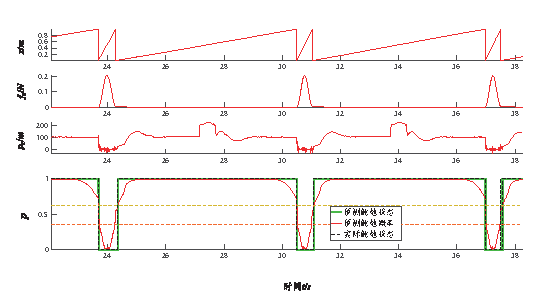
\includegraphics[width=1.\linewidth]{contact_est.eps}
    \caption{\label{fig:contact_est}触地估计示意图}
\end{figure}
\aref{fig:contact_est}展示了上述算法的实验结果。
\section{质心状态估计}
\label{sec:com_est}
包括人形机器人在内的腿足机器人有驱动关节,但并没有和环境刚性固定。因此驱动关节的角度并不能决定机器人相对环境的位姿。
腿足机器人的构型还需要确定六个自由度,通常是一个特殊的连杆相对某个惯性系的位置和姿态。这个连杆就是所谓的浮动基。
器人每个连杆的位置可以用浮动基的位姿和编码器测量得到的关节角度重建出来。

由于浮动基的状态并不是直接可测的,所以快速可靠的状态估计是在腿足机器人上实现状态反馈控制非常重要的一环。如果能知道触地点的精确位置,
那么关节的角度就足够重建出浮动基的位姿。但实际上接触很有可能会发生打滑,或者是踩到边缘脚板翻转,而且环境可能是不规则的,
机器人的几何模型中也可能有不确定性(比如柔性零件引起的变形)。因此关节角度信息是不足以实现可靠的状态估计的。

惯性测量单元(IMU)可以帮忙解决这个问题IMU通常会提供安装位置处的姿态角,角速度和线加速度。

% 最近的方法集中在融合IMU信息,力传感器数据和运动学测量来实现高保真的状态估计。IMU和运动学数据的融合最开始是用来实现里程计[1][2]。
% 之后,融合两者的高频率状态估计被用来估计速度并给闭环控制器使用:这可以在运动学层面进行[3][4][5],也可以扩展到动力学模型[6][7]。
% 其他传感器包括激光雷达的数据也可以被融合进来[8]。这些方法的共性是,解一个全耦合的推理问题来从传感器测量中估计位置和姿态。
% 然而这种全耦合的推理计算十分耗时,同时很难调参,并且通常代码实现和debug是很复杂的。

% 也有更简单的状态估计器和平衡控制器一起被提出,并且通常可以实现很震撼的实物效果[9][10][11][12][13]。这些估计器将姿态和位置估计解耦
% 来简化问题,这就引出了一个问题:为了实现高性能的控制效果,我们在多大程度上需要全耦合的位姿解算?现在还很难回答这个问题,因为这些方法
% 的严格验证有限,并且从来没有进行过合适的基准测试/对比试验(have never been properly benchmarked)。

这篇文章的主要贡献在于在WuKong4上进行了原地平衡和行走实验,并且对比(benchmark)了两种简单的状态估计方法。对比试验同样考察了不同传感器
的贡献度,比如IMU数据的加入,以及用力传感器来检测接触扰动。我们在第二和第三部分提出了两种不同的简化状态估计方法;
第四部分展示并讨论了实验结果;第五部分给出了实验结论。

\subsection{位置速度线性卡尔曼滤波器}
扩展卡尔曼滤波在人形和四足机器人的浮动基状态估计上取得了很好的效果。尽管在很多实例中EKF类的方法都表现很好,但它们的误差动力学缺乏稳定性的保证,
并且在实际中可能很难调整参数。本章使用的状态估计方法利用卡尔曼滤波实现了自适应权重的调整,从而得到浮动基的速度和位置估计。
浮动基状态估计能在一个轻微的假设下分解成分级的姿态和位置滤波器,位置和速度估计就转化成了一个线性的问题,我们就能用线性卡尔曼滤波器来处理这个问题。

\subsection{预测——过程模型}

首先我们将机器人足的位置也包括进机器人的位置和速度估计的状态量$\boldsymbol{x}$中去:
\begin{equation}
    \label{equ:est_posvel}
    \boldsymbol{x}=\left[{ }^\mathcal{I} \boldsymbol{p}_b^{\top},{ }^\mathcal{I} \boldsymbol{v}_b^{\top},{ }^\mathcal{I} \boldsymbol{p}_L^{\top},{ }^\mathcal{I} \boldsymbol{p}_R^{\top}\right]^{\top}
\end{equation}
对于$n$时刻的加速度测量$\boldsymbol{a}_n$,浮动基的位置和速度的演化可以表示为:
\begin{equation}
    \label{equ:est_posvel}
    \boldsymbol{x}_{n+1}=\left[\begin{array}{c}
        { }^{\mathcal{I}} \boldsymbol{p}_{b, n}+{ }^{\mathcal{I}} \boldsymbol{v}_{b, n} \Delta t+\frac{1}{2}\left[{ }^{\mathcal{I}} \boldsymbol{R}_{b, n} \boldsymbol{a}_n+g\right](\Delta t)^2 \\
        { }^{\mathcal{I}} \boldsymbol{v}_{b, n}+\left[{ }^{\mathcal{I}} \boldsymbol{R}_{b, n} \boldsymbol{a}_n+g\right] \Delta t \\
        { }^{\mathcal{I}} \boldsymbol{p}_{L, n} \\
        { }^{\mathcal{I}} \boldsymbol{p}_{R, n}
        \end{array}\right]
\end{equation}
我们假设每支脚和地面都是保持静止的。

通常,如果${ }^{\mathcal{I}} \boldsymbol{R}_{b}$的估计是和$\boldsymbol{x}$同时进行的,那么状态估计是在一段非线性的离散时间间隔内实现的。
然而如果近似将${ }^{\mathcal{I}} \boldsymbol{R}_{b}$的估计与$\boldsymbol{x}$的估计解耦,
那么将${ }^{\mathcal{I}} \boldsymbol{R}_{b, n} \boldsymbol{a}_n+g$看成是时变的控制输入 ,则过程模型\aref{equ:est_posvel}就变成了线性时不变的模型。

我们用了基于IMU的姿态估计器来估计${ }^{\mathcal{I}} \boldsymbol{R}_{b}$。我们使用了[14]中提出估计的第二种版本。
原本的估计器是设计来使用地磁计的,我们用运动学得到的浮动基姿态估计替换了地磁计信息。

\subsection{校正——测量模型}

为了估计$\boldsymbol{x}$,需要用运动学测量得到IMU相对脚的位置。除此之外,脚的高度$z_L$和$z_R$(这里假设为0)也被用作伪测量:
\begin{equation}
    \label{equ:est_posvel_mea}
    \boldsymbol{y}=\left[\begin{array}{c}
        { }^{\mathcal{I}} \boldsymbol{R}_b{ }^b \boldsymbol{p}_L\left(\boldsymbol{q}_L\right) \\
        { }^{\mathcal{I}} \boldsymbol{R}_b{ }^b \boldsymbol{p}_R\left(\boldsymbol{q}_R\right) \\
        z_L \\
        z_R
        \end{array}\right]
\end{equation}
通过解耦状态${ }^{\mathcal{I}} \boldsymbol{R}_{b}$的估计,它的估计值可以代入$\boldsymbol{y}$。
这种方法可以在估计测量值$\hat{\boldsymbol{y}}$和估计状态值$\hat{\boldsymbol{x}}$中建立起线性的关系:
\begin{equation}
    \label{equ:est_mea_model}
    \hat{\boldsymbol{y}}=\left[\begin{array}{c}
        { }^{\mathcal{I}} \hat{\boldsymbol{p}}_b-{ }^{\mathcal{I}} \hat{\boldsymbol{p}}_L \\
        { }^{\mathcal{I}} \hat{\boldsymbol{p}}_b-{ }^{\mathcal{I}} \hat{\boldsymbol{p}}_R \\
        \hat{z}_L \\
        \hat{z}_R
        \end{array}\right]:=\boldsymbol{C} \hat{\boldsymbol{y}}
\end{equation}
\subsection{腿部运动学噪声模型}
基于上文的解耦假设,$\boldsymbol{x}$的估计可以写成随机过程下的标准线性卡尔曼滤波:
\begin{equation}
    \label{equ:std_kf}
    \begin{aligned}
        \boldsymbol{x}_{n+1} & =\boldsymbol{A} \boldsymbol{x}_n+\boldsymbol{B} u_n+\mathcal{N}\left(0, \boldsymbol{Q}_n\right) \\
        \boldsymbol{y}_{n+1} & =C \boldsymbol{x}_{n+1}+\mathcal{N}\left(0, \boldsymbol{R}_{n+1}\right)
        \end{aligned}
\end{equation}
$A$和$B$满足\aref{equ:est_posvel},$\boldsymbol{Q}_n$和$\boldsymbol{R}_n$分别是过程噪声和测量噪声的协方差矩阵。为了正确地表示支撑相和摆动相之间的切换,我们设计了一种根据腿的触地状态
来调整腿部运动学信息的噪声大小。

我们用$\rho_{trust}$来表示某一条腿的运动学信息的可信度,由于我们的预测模型假设腿和地面是相对静止的,因此摆动腿运动学信息的可信度为0,摆动腿的相位和可信度$\rho_{trust}$的关系如\aref{fig:kin_trust}。
在支撑相刚开始和即将结束时,支撑腿可能未站稳,和地面有相对滑动的可能增加,其运动学信息的可信度降低,因此这种函数关系是符合直觉的。这里我们用信任窗口$trustWindow$值的大小来表示支撑相“刚开始”和“要结束”的状态具体有多长。
\begin{figure}[htbp]
    \centering
    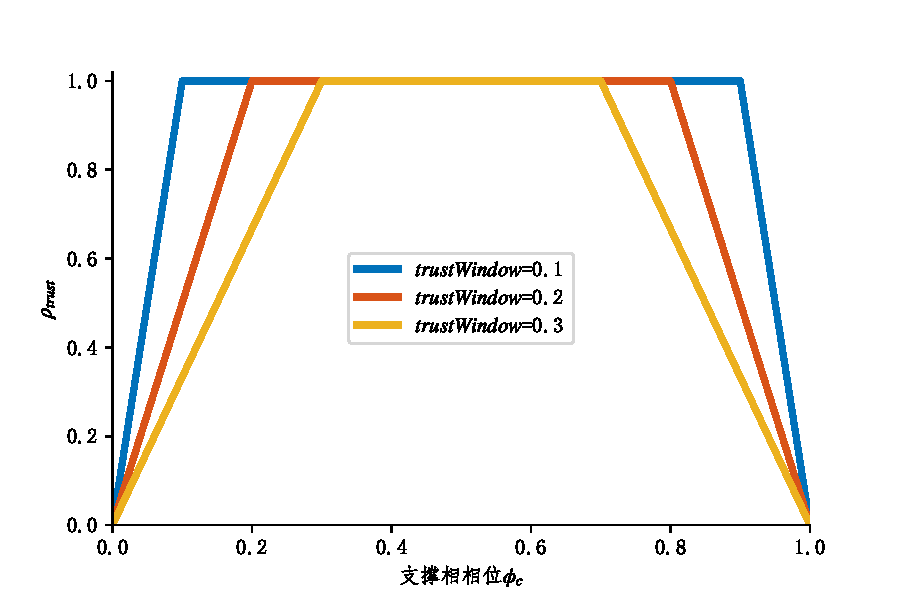
\includegraphics[width=1.\linewidth]{trust.pdf}
    \caption{\label{fig:kin_trust}支撑腿运动学信息可信度随相位变化图}
\end{figure}

运动学测量的方差根据可信度$\rho_{trust}$计算,随后用标准卡尔曼滤波的更新方程来得到浮动基位置和速度估计,具体的算法流程在\aref{alg:com_state_est}中给出。
\begin{algorithm}[htb]
\setstretch{1.3}
\caption{质心状态估计迭代过程} 
\label{alg:com_state_est} 
\begin{algorithmic}[1] %这个1 表示从第一行开始显示行号,不写就不会显示行号
\STATE{\fangsong{\textbf{输入}}:$\hat{\boldsymbol{x}}_{k-1}, \tilde{\boldsymbol{z}}_k, \boldsymbol{\Sigma}_{k-1}, \boldsymbol{Q}_{w_k}, \boldsymbol{R}_{v_k}, \phi$}
\STATE{\fangsong{\textbf{输出}}:$\hat{\boldsymbol{x}}_{k}, \tilde{\boldsymbol{z}}_k, \boldsymbol{\Sigma}_{k}$}
\STATE{\textbf{Step 1}\ \fangsong{初始化}$\boldsymbol{A}_0, \boldsymbol{B}_0, \boldsymbol{H}_0, \boldsymbol{Q}_0,\boldsymbol{R}_0, \boldsymbol{\Sigma}_0,Noise$}
\STATE{$\ \ \ \ \ \ \ \ \ \ \ \ \ \ \ \ \boldsymbol{x}_0=\left[{ }^\mathcal{I} \boldsymbol{p}_{b,0}^{\top},{ }^\mathcal{I} \boldsymbol{v}_{b,0}^{\top},{ }^\mathcal{I} \boldsymbol{p}_{L,0}^{\top},{ }^\mathcal{I} \boldsymbol{p}_{R,0}^{\top}\right]^{\top}$}
\STATE{\textbf{Step 2}\ \fangsong{更新每条腿运动学信息的噪声}:}
\FOR{$i=0, 1$}
\STATE{$\begin{aligned}
    id &= 3 \times i\\
    q_{id} &= 6 + id\\
    r_{id1} &= id\\
    r_{id2} &= 6 + id\\
    r_{id3} &= 12 + i
\end{aligned}$
}
\IF{$\phi \le 0.2$}
\STATE{$\rho_{trust}=\phi / 0.2$}
\ELSIF{$\phi > 0.8$}
\STATE{$\rho_{trust}=(1-\phi) / 0.2$}
\ENDIF
\STATE{$\begin{aligned}
        \boldsymbol{Q}.block(q_{id}, q_{id}, 3, 3) &= (1 + Noise * (1 - \rho_{trust})) * \boldsymbol{Q}.block(q_{id}, q_{id}, 3, 3)\\
        \boldsymbol{R}.block(r_{id2}, r_{id2}, 3, 3) &= (1 + Noise * (1 - \rho_{trust})) * \boldsymbol{R}.block(r_{id2}, r_{id2}, 3, 3)\\
        \boldsymbol{R}(r_{id3}, r_{id3}) &= (1 + Noise * (1 - \rho_{trust})) * \boldsymbol{R}(r_{id3}, r_{id3})
        \end{aligned}$}
\ENDFOR
\STATE{\textbf{Step 3}\ \fangsong{预测}:}
\STATE{$\ \ \begin{gathered}
        \hat{\boldsymbol{x}}_{k \mid k-1}=\boldsymbol{A}_k \hat{\boldsymbol{x}}_{k-1}+\boldsymbol{B}_k \boldsymbol{u}_k \\
        \boldsymbol{\Sigma}_{k \mid k-1}=\boldsymbol{A}_k \boldsymbol{\Sigma}_{k-1} \boldsymbol{A}_k^T+\boldsymbol{Q}_{w_k}
        \end{gathered}$}
\STATE{\textbf{Step 4}\ \fangsong{计算卡尔曼增益}:}
\STATE{$\ \ \boldsymbol{K}_k=\boldsymbol{\Sigma}_{k \mid k-1} \boldsymbol{H}_k^T\left(\boldsymbol{H}_k \boldsymbol{\Sigma}_{k \mid k-1} \boldsymbol{H}_k^T+\boldsymbol{R}_{v_k}\right)$}
\STATE{\textbf{Step 5}\ \fangsong{校正}:}
\STATE{$\ \ \begin{aligned}
    \hat{\boldsymbol{x}}_{k \mid k}&=\hat{\boldsymbol{x}}_{k \mid k-1}+\boldsymbol{K}_k\left(\tilde{\boldsymbol{z}}_k-\boldsymbol{H}_k \hat{\boldsymbol{x}}_{k \mid k-1}\right) \\
    \boldsymbol{\Sigma}_{k \mid k}&=\left(\mathbf{I}-\boldsymbol{K}_k \boldsymbol{H}_k\right) \boldsymbol{\Sigma}_{k \mid k-1}
    \end{aligned}$}

\end{algorithmic}
\end{algorithm}
\section{实物实验}
借助动作捕捉系统,我们验证了质心位置估计的准确性。实验环境如\aref{fig:capture_exp}所示,对比行走过程中质心位置估计结果和动作捕捉的数据(\aref{fig:com_pos_est}),可以看出二者基本相符。
图中虚线内的部分是由于机器人走到了动捕镜头的盲区,所以出现了较大的偏差。
\begin{figure}[htbp]
    \centering
    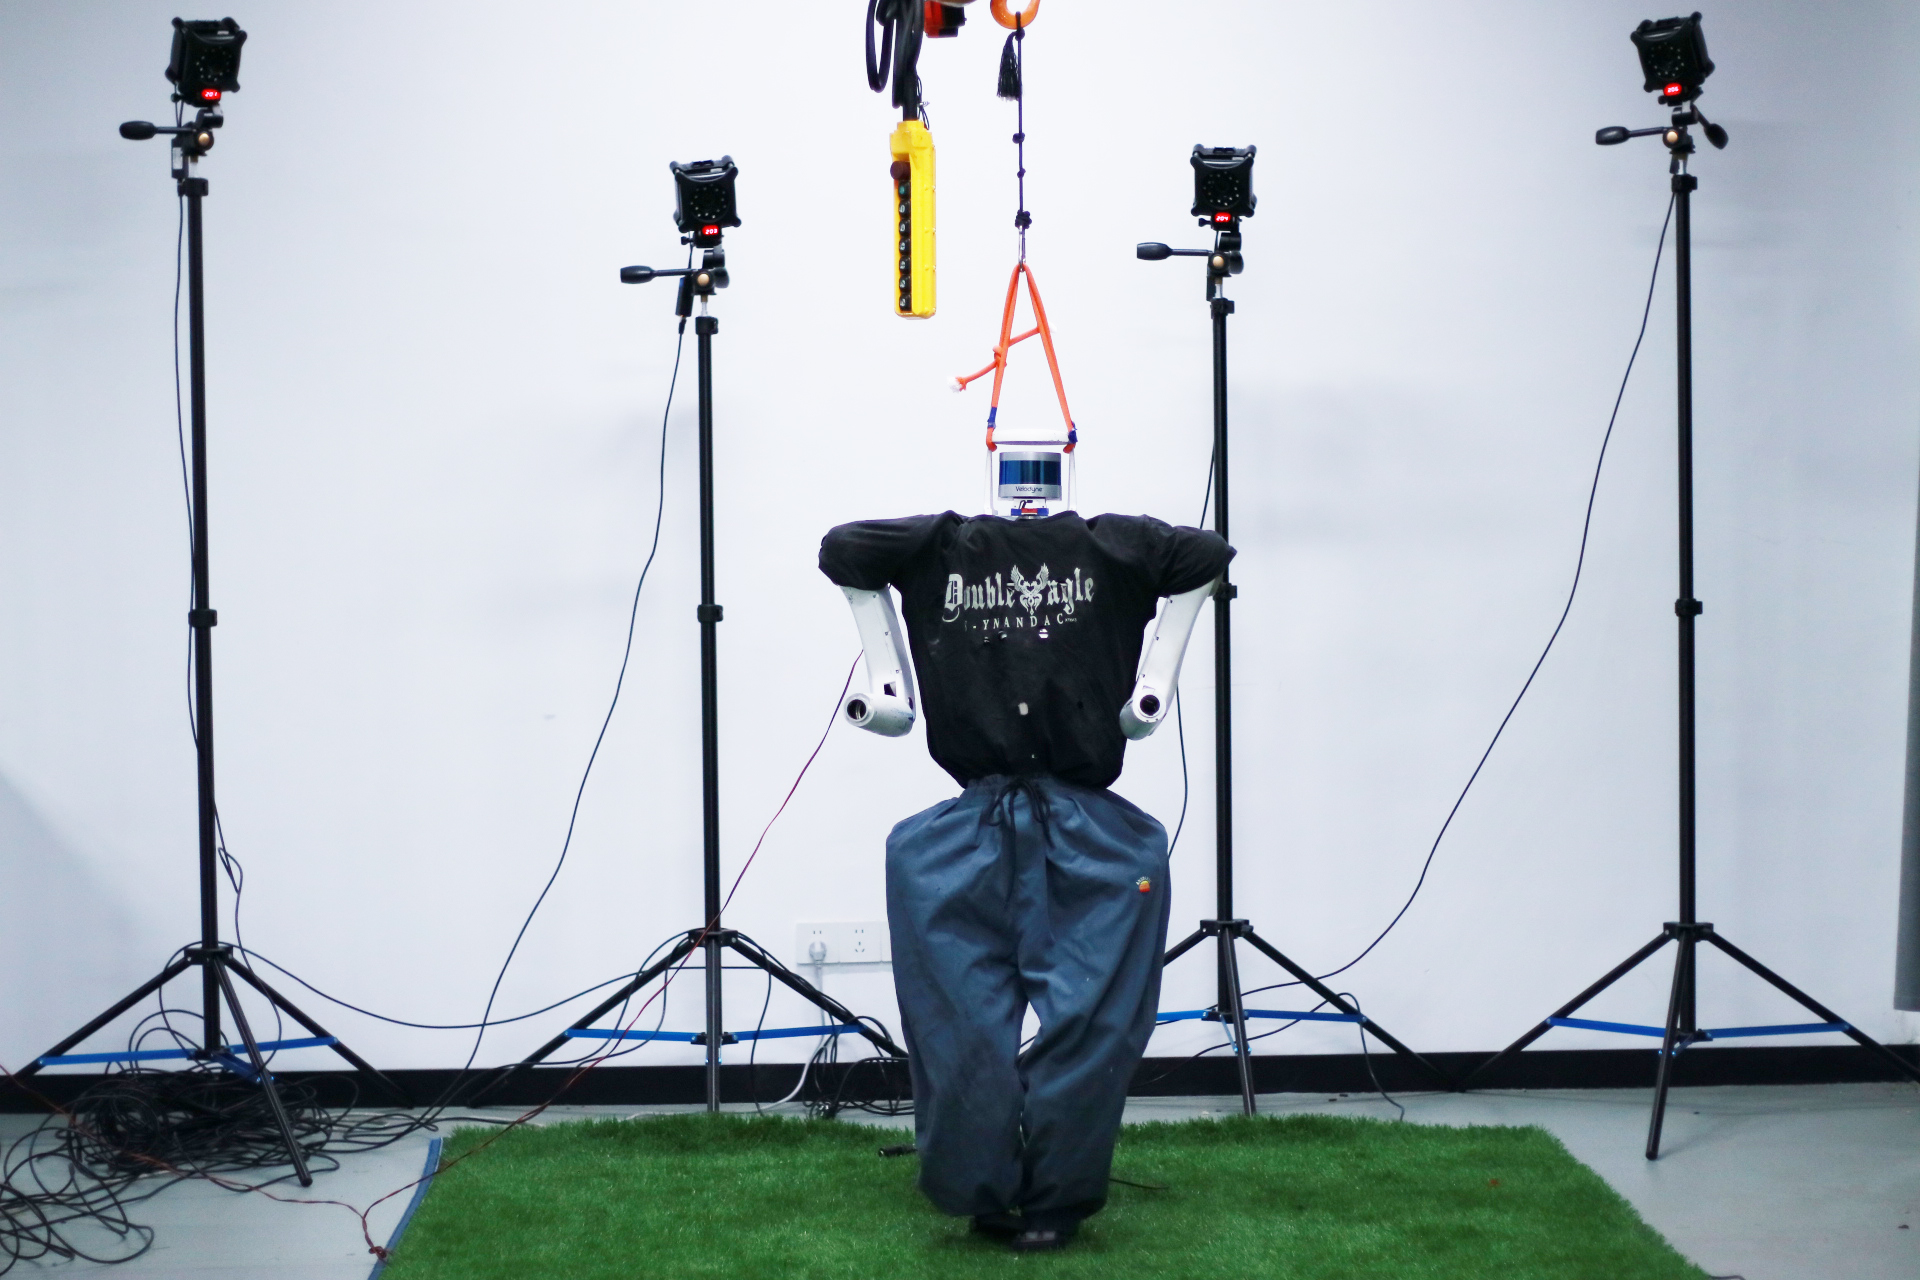
\includegraphics[width=.8\linewidth]{动捕.jpg}
    \caption{\label{fig:capture_exp}动作捕捉实验图}
\end{figure}

\begin{figure}[htbp]
    \centering
    \includegraphics[width=1.\linewidth]{rectangle.pdf}
    \caption{\label{fig:com_pos_est}质心位置估计结果}
\end{figure}

\chapter{基于二次规划的仿人机器人运动控制器}
本章提出了针对浮动基机器人的一种基于动量的控制架构,并在仿人机器人WuKong-IV上进行了实现。该控制架构的核心是一个二次规划问题,
该二次规划问题协调了用关节加速度向量的约束表达的运动任务,以及单边的地面接触约束和摩擦约束、关节力矩约束带来的限制。
该架构在实际硬件平台上得到了验证,可以实现仿人机器人的高速稳定行走,和对期望轨迹的稳定跟随。
\section{实验平台介绍}
\begin{figure}[htbp]
    \centering
    \subcaptionbox{正视图\label{subfig:wukong_front}}
        {%
            \includegraphics[height = .5\linewidth]{正视图.png}}
    \subcaptionbox{侧视图\label{subfig:wukong_side}}
        {%
            \includegraphics[height = .5\linewidth]{侧视图.png}}
    \caption{WuKong-IV仿人机器人实物样机\label{fig:wukong_pic}}
\end{figure}
本文研究基于仿人机器人WuKong-IV实验平台实现,实物图见\aref{fig:wukong_pic},WuKong-IV双
足机器人是浙江大学研发的仿人仿人机器人移动实验平台。机器人身高约1.5m,重约
46kg,其中大腿连杆长度为0.3m,小腿连杆长度0.3m。全身共有21个自由度,其中
左腿与右腿各有6个自由度,腰关节有1个自由度,左手臂与右手臂各有4个自由度。
其中每条腿的髋关节部分有3个自由度,按照关节旋转方向将髋关节3个自由度命名为
髋关节侧摆关节,髋关节俯仰关节,髋关节偏航关节。机器人膝关节有1个
自由度,踝关节有两个自由度。机器人腿部的每个自由度均由高能量密度的无刷直流电机执行,采用“大力矩
电机+低减速比”结构,腰关节采用的为高转速力矩电机。其中踝关节电机采用了连杆结构,
其余关节电机均采用齿轮减速器,减速比恒定不变,腿部各关节电机与关节信息见\aref{joint_motor}。
\begin{table}[htbp]
	\centering
    \setstretch{1.3}
	\caption{WuKong-IV仿人机器人各关节信息}
	\label{joint_motor}
	\begin{tabular}{m{3cm}<{\centering}m{3cm}<{\centering}m{1.5cm}<{\centering}m{2cm}<{\centering}m{2.5cm}<{\centering}}
		\toprule  %添加表格头部粗线
		关节名称   &电机型号  &减速比  &输出最大力矩/$N \cdot m$ &关节额定转速/$rad\cdot s^{-1}$ \\
		\midrule  %添加表格中横线
		膝关节 & 105ZWS04 & 12 & 180 & 12.00\\
		腰关节 & 85ZWS02 & 12 & 84.0 & 7.85\\        
		髋偏航关节 & 85ZWS02 & 12 & 84.0 & 7.85\\
		髋横滚关节 & 85ZWS02 & 12 & 84.0 & 7.85\\
		髋俯仰关节 & 85ZWS02 & 12 & 84.0 & 7.85\\
        踝横滚关节 & 60ZWS01-1J22 & 7 & 28.0 & 14.65\\
        踝横滚关节 & 60ZWS01-1J22 & 7 & 28.0 & 14.65\\
        手臂所有关节 & 60ZWS01-1J22 & 25 & 100.0 & 4.1\\
		\bottomrule %添加表格底部粗线
	\end{tabular}
\end{table}
\subsection{坐标系定义}
\begin{figure}[!htbp]
    \centering
    \includegraphics[width=.8\linewidth]{关节构型.eps}
    \caption{\label{fig:centroid}仿人机器人坐标系定义}
\end{figure}
在\aref{fig:centroid}定义的机器人坐标系下,按照每个关节的旋转轴方向可以根据转轴分为横滚($roll$) ,
俯仰($pitch$)和偏航($yaw$)三种,因此可以将全部的关节根据基于前一个连杆的旋转角
度方向定义为横滚角关节、俯仰角关节和偏航角关节。同时定义机器人坐标系下$x$轴、
$y$轴方向为机器人运动的正方向和左方向;机器人躯干的向前俯仰为正角度,向右横滚
为正角度,向左偏航为正角度。

在世界坐标系下,定义机器人身体姿态角为绕机器人坐标系坐标轴转动的角度,也
就是机器人坐标系相对于世界坐标系的旋转角度;定义机器人的质心高度为世界坐标系
下质心在$z$轴方向的位置;定义质心速度为世界坐标系下机器人的$x$轴和$y$轴方向的速
度,定义摆动腿的落脚点和摆动轨迹为机器人坐标系下摆动腿的位置。
\subsection{简化连杆模型}

实物机器人有着较为复杂的连杆关系与机械结构,为了方便运动学和动力学的运算,
本文将WuKong-IV仿人机器人的机械结构简化成多连杆模型,如图所示。由于两款机器
人的简化连杆模型除了连杆长度参数不一致以外其他基本一致,因此两款机器人可以采
用同一套多连杆模型。关节命名的顺序就是从上文定义的质心位置开始往外延伸依次定
义。关节0表示腰偏航关节,关节1, 2, 3分别表示左腿髓偏航、左腿髓横滚、左腿髓
俯仰关节,关节4表示左腿膝关节,关节5, 6表示左腿跺横滚、左腿跺俯仰关节,关
节7,  8,   9表示右腿髓偏航关节、右腿髓横滚、右腿髓俯仰关节,关节10表示右腿膝
关节,关节11, 12表示右腿跺横滚、右腿跺俯仰关节,关节13, 14, 15表示左肩偏航、
左肩横滚、左肩俯仰关节,关节16表示左肘俯仰关节,关节17, 18, 19表示右肩偏航、
右肩横滚、右肩俯仰关节,关节20表示右肘俯仰关节。简化的全身连杆模型2.6如图所
示。在计算运动学方面各种方法可以都直接采用该简化连杆模型。而在考虑动力学的时
候,如果是解祸控制的方法,由于上半身动作在该模型当中对于全身没有影响,基本上
采用的是不包括上半身的简化模型。与此同时由于全身大多数惯量也都集中在质心的位
置,所以也可以大概的将腿部的连杆理解成质量为0的连杆。
% 但对于采用全身控制和模
% 型预测控制的方法来讲,由于考虑了动力学约束所以可以兼顾考虑上半身的影响,因而
% 往往需要采用全身连杆模型。

\begin{figure}[htbp]
    \centering
    \includegraphics[width=.4\linewidth]{简化连杆.eps}
    \caption{\label{fig:link_model}WuKong-IV仿人机器人的简化连杆模型}
\end{figure}
\section{仿人机器人动力学建模与控制器设计}

% 本文提出了针对浮动基机器人的一种基于动量的控制架构,并在仿人机器人Atlas上进行了实现。该控制架构的核心是一个二次规划问题,
% 该二次规划问题协调了用关节加速度向量的约束表达的运动任务,和单边的地面接触和有限的抓地力(force-limited grasping)带来的限制。
% 我们竭力做了一些必要的改动,使得该架构可以从仿真环境移植到实际硬件平台上,并且提出了机器人走过复杂地形,一些基本的操作任务,
% 以及在斜面上的多接触点平衡(后者仅在仿真中实现)。
\subsection{质心动力学}
\begin{figure}[htbp]
    \centering
    \includegraphics[width=.8\linewidth]{质心模型.eps}
    \caption{\label{fig:com_model}WuKong-IV仿人机器人质心模型}
\end{figure}
% 这部分简要地回顾了机器人的质心动力学的一些关键性质。对于更深层次的讨论,见[25]。
% 在本文中,
我们把机器人看作刚体,其有广义关节力矩向量$\tau \in {{\mathbb{R}}^{n}}$,关节构型向量$q\in {{\mathbb{R}}^{m}}$,
关节速度向量$v\in {{\mathbb{R}}^{n+6}}$(区分$v$和$\dot q$是为了用关节构型的冗余参数来避免奇异问题(比如使用欧拉角而不是$rpy$来表示浮动基姿态),
同时使用最少的参数来表示速度向量(比如使用角速度而不是四元数的导数))。我们假设机器人和世界系之间的“浮动关节”是唯一的无驱动自由度。令
\begin{equation}
    \label{equ:momentum}
    \boldsymbol{h}=\left(\begin{aligned}
        & \boldsymbol{k} \\ 
       & \boldsymbol{l} \\ 
      \end{aligned} \right)\in \mathbb{R}^{6}
\end{equation}
表示机器人的质心动量,$\boldsymbol{k}\in {{\mathbb{R}}^{3}}$表示质心角动量,$\boldsymbol{l}\in {{\mathbb{R}}^{3}}$
表示质心线动量(符号表示采用[25])。“质心”表示所有的量都在质心系下表示,质心系和世界系有同样方向的坐标轴,但其原点在机器人的瞬时质心处。
机器人的质心动量就等于所有连杆在质心系下的动量之和。众所周知,无论机器人有多复杂,其质心动力学都是简单的。
欧拉定律表明机器人的质心动量的变化率就等于施加在机器人上的所有外部力旋量之和。可以写成:
\begin{equation}
    \label{equ:euler's_law}
    \dot{\boldsymbol{h}}={{\boldsymbol{W}}_{g}}+\sum\limits_{i}{{{\boldsymbol{W}}_{gr,i}}}+\sum\limits_{i}{{{\boldsymbol{W}}_{ext,i}}}
\end{equation}
	
其中${{\boldsymbol{W}}_{g}}={{[\mathbf{0}_{3\times 1}^{\top }\ \ m{{\mathbf{g}}^{\top }}]}^{\top }}$表示重力矩,
${\boldsymbol{W}}_{gr,i}$表示由于机器人刚体和环境接触产生的环境作用力旋量,${\boldsymbol{W}}_{ext,i}$表示机器人受到的接触力和重力之外的
其它外部力旋量。注意机器人系统的动量变化率和内部力或者力矩无关。
% Orin和Goswami指出关节速度向量$v$和机器人的质心动量之间存在着简单的线性关系[2]
\begin{equation}
    \label{equ:euler_linear_equ}
    \boldsymbol{h}=\boldsymbol{A}(q)\boldsymbol{v}
\end{equation}
其中$boldsymbol{A}(q)$被称作质心动量矩阵(centroidal momentum matrix,CMM)。将\aref{equ:euler_linear_equ}代入\aref{equ:euler's_law}可以得到
\begin{equation}
    \label{equ:euler_wrench}
    \boldsymbol{A}\dot{\boldsymbol{v}}+\dot{A}v={{\boldsymbol{W}}_{g}}+\sum\limits_{i}{{{\boldsymbol{W}}_{gr,i}}}
    +\sum\limits_{i}{{{\boldsymbol{W}}_{ext,i}}}
\end{equation}
\aref{equ:euler_wrench}表明关节加速度向量$\dot{\boldsymbol{v}}$和机器人受到的力旋量之间存在仿射关系,我们在后续的控制架构中利用了这一点。

\subsection{控制架构}
\begin{figure}[htbp]
    \centering
    \includegraphics[width=1.\linewidth]{qp控制框架.eps}
    \caption{\label{fig:framework_control_flow}控制架构中上层信息流概览}
\end{figure}
\aref{fig:framework_control_flow}展示了我们的控制架构的上层信息流。一个上层的运动行为,比如行走或者开车行为,
用下列数据构建了一个二次规划问题:
1)	运动任务(motion task)形式的期望运动;
2)	可行接触的信息;
3)	期望质心动量的变化率。
QP利用\aref{equ:euler_wrench}协调运动任务和可行接触。QP求解器输出关节加速度和与环境接触的连杆所受的环境接触力。
这些信息随后通过一种逆动力学算法来计算期望的关节力矩。计算出的力矩随后用来确定发送给机器人关节电机的力矩指令。
\subsubsection{期望运动}
在我们的架构中,运动任务是用来确定期望的机器人运动的。运动(motion)是动量变化率方程\aref{equ:euler_wrench}等式左边的部分。
我们将运动任务定义为和机器人期望的广义速度向量线性相关的方程,${\dot{\boldsymbol{v}}}_{d}\in {\mathbb{R}}^{(n+6)}$,
包括了机器人浮动基关节相对于世界系的空间加速度。$n$是驱动关节的数量。第$i$个运动任务可以写成
\begin{equation}
    \label{equ:motion_task}
    \boldsymbol{J}_i \dot {\boldsymbol{v}}_d = \boldsymbol{p}_i
\end{equation}


% \subsubsection{外部力旋量}
% 本节是关于动量变化率方程\aref{equ:euler_wrench}的等式右边:外部力旋量。地面作用旋量${\boldsymbol{W}}_{gr,i}$由特定约束下的QP中的决策变量参数化。
% 两种形式的地面接触是可行的:单边地面接触(4.2.1)和有限抓地力接触(4.2.2)。其他的待补偿的外部力旋量 在4.2.3中讨论。
\subsubsection{单边地面接触}
单边地面接触被建模成有静摩擦力的点接触。有分布的负载的平的,多边形的接触面可以被等效地建模成顶点处的点接触。
对于法向量为${{\boldsymbol{n}}_{i}}$的第$i$个点接触,接触力${{\boldsymbol{f}}_{i}}$的摩擦约束可以写成:
\begin{equation}
    \label{equ:friction_cone}
    \left\| {{\boldsymbol{f}}_{i}}-({{\boldsymbol{n}}_{i}}{{\boldsymbol{f}}_{i}}){{\boldsymbol{n}}_{i}} \right\|\le \mu {{\boldsymbol{n}}_{i}}{{\boldsymbol{f}}_{i}}
\end{equation}
其中$\mu$是摩擦系数。\aref{equ:friction_cone}的二阶锥约束不能结合到一个二次规划中,并且二阶锥规划(SOCP)还没有比较快的求解器,
所以我们用了标准的保守对摩擦锥的多棱锥(polyhedral)近似。近似出的摩擦锥用原本的二阶锥的一组$m$个射线作为基向量来参数化(如\aref{fig:friction_cone}),
即我们用下式来替代\aref{equ:friction_cone}:
\begin{equation}
    \label{equ:friction_para}
    \begin{aligned}
        & {{\boldsymbol{f}}_{i}}=\sum\limits_{j=1}^{m}{{{\rho }_{ij}}{{\boldsymbol{\beta}}_{ij}}} \\ 
       & {{\rho }_{ij}}\ge 0 \\ 
      \end{aligned}      
\end{equation}
其中$\boldsymbol{\beta}_{ij} \in \mathbb{R}^3$是基向量,$\rho_{ij}$是坐标。在本文提出的结果中我们用了四个基向量,将$\mu$设为0.8。
\begin{figure}[htbp]
    \centering
    \includegraphics[width=.8\linewidth]{摩擦锥.eps}
    \caption{\label{fig:friction_cone}质心系下$\boldsymbol{r}_{i}$处法向量为${{\boldsymbol{n}}_{i}}$的单边接触,摩擦锥由基向量$\boldsymbol{\beta}_{ij}$近似}
\end{figure}
质心系下的地面接触力旋量${{\boldsymbol{W}}_{gr,i}}$和接触力${{\boldsymbol{f}}_{i}}$的关系可以表示成:
\begin{equation}
    \label{equ:contact_wrench}
    {\boldsymbol{W}_{gr,i}}=\left( \begin{aligned}
        & {{{\hat{\boldsymbol{r}}}}_{i}} \\ 
       & I \\ 
      \end{aligned} \right){\boldsymbol{f}_{i}}      
\end{equation}
其中${\boldsymbol{r}_{i}}$表示质心系下接触点$i$的位置,${{\hat{\boldsymbol{r}}}_{i}}\in {{\mathbb{R}}^{3}}$是满足
${{\hat{\boldsymbol{r}}}_{i}}{\boldsymbol{f}_{i}}\equiv {\boldsymbol{r}_{i}}\times {\boldsymbol{f}_{i}}$的反对称矩阵。
将\aref{equ:friction_para}与\aref{equ:contact_wrench}结合,可以得到
\begin{equation}
    \label{equ:wrench_matrix}
    \begin{aligned}
        & {{\boldsymbol{W}}_{gr,i}}={{\boldsymbol{Q}}_{i}}{{\boldsymbol{\rho}}_{i}} \\ 
       & {{\boldsymbol{\rho}}_{i}}\ge 0 \\ 
      \end{aligned}        
\end{equation}
其中,${{\boldsymbol{Q}}_{i}}=\left[ \begin{aligned}
    & {{{\hat{\boldsymbol{r}}}}_{i}}{{\boldsymbol{\beta}}_{i1}} \\ 
   & {{\boldsymbol{\beta}}_{i1}}\ \ \ \  \\ 
  \end{aligned} \right.\ \ \ \ \cdots \ \ \ \ \left. \begin{aligned}
    & {{{\hat{\boldsymbol{r}}}}_{i}}{{\boldsymbol{\beta}}_{im}} \\ 
   & {{\boldsymbol{\beta}}_{im}} \\ 
  \end{aligned} \right]
  $。
  实际我们用了和接触的刚体表面固定的坐标系的面法向量${{\boldsymbol{n}}_{j}}$。
%   我们更愿意使用Pollard和Reitsma的射线参数化,
%   而不是Stewart和Trinkle的另一种参数化,因为射线参数化每个接触点要求的决策变量都会少一个。
\subsection{二次规划构建过程}

最终我们得到的二次规划问题如\ref{equ:qp_control}所示:
\begin{equation}
    \label{equ:qp_control}
    \begin{aligned}
       \underset{{{{\dot{\boldsymbol{v}}}}_{\text{d}}},\boldsymbol{\rho}}{\mathop{\operatorname{minimize}}}\,\quad {{\left( \boldsymbol{A}{{{\dot{\boldsymbol{v}}}}_{\text{d}}}-\boldsymbol{b} \right)}^{\top }}&{{C}_{{\dot{\boldsymbol{h}}}}}\left( \boldsymbol{A}{{{\dot{\boldsymbol{v}}}}_{\text{d}}}-\boldsymbol{b} \right)+{{\boldsymbol{\rho} }^{\top }}{{\boldsymbol{C}}_{\boldsymbol{\rho} }}\boldsymbol{\rho} +\dot{\boldsymbol{v}}_{\text{d}}^{\top }{{\boldsymbol{C}}_{{\dot{\boldsymbol{v}}}}}{{{\dot{\boldsymbol{v}}}}_{\text{d}}} \\ 
        \text{subject to}\quad \boldsymbol{A}{{{\dot{\boldsymbol{v}}}}_{\text{d}}}+\dot{\boldsymbol{A}}\boldsymbol{v}&={\boldsymbol{{}W}_{g}}+\boldsymbol{Q}\boldsymbol{\rho} +\sum\limits_{i}{{{\boldsymbol{W}}_{\text{ext },i}}} \\ 
        \boldsymbol{J}{{{\dot{\boldsymbol{v}}}}_{\text{d}}}&=\boldsymbol{p} \\ 
        {{\boldsymbol{\rho} }_{\min }}&\le \boldsymbol{\rho} \le {{\boldsymbol{\rho} }_{\max }} 
      \end{aligned}
\end{equation}
其中,$\boldsymbol{b}={{\dot{\boldsymbol{h}}}_{d}}-\dot{\boldsymbol{A}}\boldsymbol{v}$,${{\dot{\boldsymbol{h}}}_{d}}\in {{\mathbb{R}}^{6}}$表示期望的质心动量变化率。
${{\boldsymbol{C}}_{{\dot{\boldsymbol{h}}}}},{\boldsymbol{{C}}_{\boldsymbol{\rho} }},{\boldsymbol{C}_{{\dot{\boldsymbol{v}}}}}$是由更上层的控制器决定的目标函数权重矩阵。\aref{tab:qp_weight}给出了行走行为下的权重矩阵示例。
\begin{table}[htbp]
    \setstretch{1.3}
	\centering
	\caption{权重矩阵的数值}
	\label{tab:qp_weight}
	\begin{tabular}{m{2cm}<{\centering}m{2cm}<{\centering}}
		\toprule  %添加表格头部粗线
		\fangsong{参数名称}   &数值  \\
		\midrule  %添加表格中横线
		${{\boldsymbol{C}}_{{\dot{\boldsymbol{h}}}}}$    & $\mathbf{I}$\\
		${\boldsymbol{{C}}_{\boldsymbol{\rho} }}$ &  $0.01 \mathbf{I}$ \\
		${\boldsymbol{C}_{{\dot{\boldsymbol{v}}}}}$ & $0.05 \mathbf{I}$ \\
		\bottomrule %添加表格底部粗线
	\end{tabular}
\end{table}
二次规划问题构建的具体算法流程由\aref{alg:quadratic_program}给出,最终我们使用了pOASES求解库来进行问题的数值求解,平均求解时间在2ms左右。
\begin{algorithm}[htb] 
\setstretch{1.3}
\caption{二次规划问题构建过程} 
\label{alg:quadratic_program} 
\begin{algorithmic}[] %这个1 表示从第一行开始显示行号,不写就不会显示行号
\STATE{$\underset{{{{\dot{\boldsymbol{v}}}}_{\text{d}}},\boldsymbol{\rho}}{\mathop{\operatorname{minimize}}}\,\quad {{\left( \boldsymbol{A}{{{\dot{\boldsymbol{v}}}}_{\text{d}}}-\boldsymbol{b} \right)}^{\top }}{{C}_{{\dot{\boldsymbol{h}}}}}\left( \boldsymbol{A}{{{\dot{\boldsymbol{v}}}}_{\text{d}}}-\boldsymbol{b} \right)+{{\boldsymbol{\rho} }^{\top }}{{\boldsymbol{C}}_{\boldsymbol{\rho} }}\boldsymbol{\rho} +\dot{\boldsymbol{v}}_{\text{d}}^{\top }{{\boldsymbol{C}}_{{\dot{\boldsymbol{v}}}}}{{{\dot{\boldsymbol{v}}}}_{\text{d}}}$}
\STATE{$\bf{subject\ to:}$}
\STATE{$\boldsymbol{x}(0)=\boldsymbol{x}_0$}
\STATE{$\boldsymbol{v}(0)=\boldsymbol{v}_0$}
\FOR{$i=1...P$}
\STATE{$\begin{aligned}
    & T_i{ }^{\min } \leq T_i \leq T_i^{\max } \\
    & \mathrm{dt}_i:=T_i / N
    \end{aligned}$}
\FOR{$k=((i-1)P)...(i\cdot P-1)$}
\STATE{$\begin{aligned}
    & \boldsymbol{x}(k+1)=\boldsymbol{x}(k)+\mathrm{dt}_i \boldsymbol{v}(k)+\frac{1}{2} \mathrm{dt}_i^2 \boldsymbol{a}(k) \\
    & \boldsymbol{v}(k+1)=\boldsymbol{v}(k)+\mathrm{dt}_i \boldsymbol{a}(k) \\
    & \mathbf{a}:=-\boldsymbol{g}
    \end{aligned}$}
\STATE{$\begin{aligned}
    & \mathbf{a}:=\mathbf{a}+\lambda_l(k)\left(\boldsymbol{x}(k)-\boldsymbol{x}_{l, i}-\boldsymbol{R}_{l, i} \boldsymbol{p}_l(k)\right) \\
    & \boldsymbol{A}_{l, i} \boldsymbol{p}_l(k) \leq \boldsymbol{b}_{l, i} \\
    & {\left[1\ 1\ -\mu^2\right]\left(\boldsymbol{R}_{l, i}^{\top}\left(\boldsymbol{x}(k)-\boldsymbol{x}_{l, i}-\boldsymbol{R}_{l, i} \boldsymbol{p}_l(k)\right)\right)^2 \leq 0} \\
    & \boldsymbol{F}_{l, i} \boldsymbol{R}_{l, i}^{\top}\left(\boldsymbol{x}(k)-\boldsymbol{x}_{l, i}-\boldsymbol{R}_{l, i} \boldsymbol{p}_l(k)\right) \leq 0 \\
    & l^{\text {min }} \leq\left\|\boldsymbol{x}-\boldsymbol{x}_{l, i}\right\| \leq l^{\max }
    \end{aligned}$}
\STATE{$\boldsymbol{a}(k)=\bf{a}$}
\ENDFOR
\ENDFOR
\end{algorithmic}
\end{algorithm}
\section{行走实验}

我们在WuKong-IV实物样机上部署了上述算法,并进行了相关行走实验验证了算法的有效性。\aref{fig:track_exp}是轨迹跟踪实验的实验截图,在该实验中,
我们让机器人跟随一段规划好的五次多项式轨迹,跟踪曲线如\aref{fig:com_pos_track}所示。
\begin{figure}[htbp]
    \centering
    \includegraphics[height=.32\linewidth]{walk_1.jpg}
    \includegraphics[height=.32\linewidth]{walk_2.jpg}
    \includegraphics[height=.32\linewidth]{walk_3.jpg}
    \includegraphics[height=.32\linewidth]{walk_4.jpg}

    \includegraphics[height=.32\linewidth]{walk_5.jpg}
    \includegraphics[height=.32\linewidth]{walk_6.jpg}
    \includegraphics[height=.32\linewidth]{walk_7.jpg}
    \includegraphics[height=.32\linewidth]{walk_8.jpg}   
    \caption{\label{fig:track_exp}WuKong-IV轨迹跟踪实验截图}
\end{figure}
\begin{figure}[htbp]
    \centering
    \includegraphics[width=.8\linewidth]{rectangle_track.pdf}
    \caption{\label{fig:com_pos_track}质心位置跟踪曲线}
\end{figure}
除此之外,我们还通过快速行走实验验证了上述算法在高速场景下的鲁棒性。实验截图如\aref{fig:track_exp}所示。由质心速度估计得到的速度曲线如\aref{fig:com_vel_track}。
\begin{figure}[htbp]
    \centering
    \includegraphics[height=.32\linewidth]{fast_walk1.jpg}
    \includegraphics[height=.32\linewidth]{fast_walk2.jpg}
    \includegraphics[height=.32\linewidth]{fast_walk3.jpg}
    \includegraphics[height=.32\linewidth]{fast_walk4.jpg}

    \includegraphics[height=.32\linewidth]{fast_walk5.jpg}
    \includegraphics[height=.32\linewidth]{fast_walk6.jpg}
    \includegraphics[height=.32\linewidth]{fast_walk7.jpg}
    \includegraphics[height=.32\linewidth]{fast_walk8.jpg}   
    \caption{\label{fig:track_exp}WuKong-IV快速行走实验截图}
\end{figure}
\begin{figure}[htbp]
    \centering
    \includegraphics[width=1.\linewidth]{velo.eps}
    \caption{\label{fig:com_vel_track}质心速度曲线}
\end{figure}
\chapter{仿人机器人质心轨迹优化}
% \section{基于二次规划的全身控制器}
% 机器人运动由基于QP的全身控制器控制[22],该控制器输出一组期望关节加速度,包括浮动基关节在惯性系$\mathcal{I}$下的空间加速度,
% 这里我们用$\dot{\boldsymbol{\nu}}_d \in \mathbb{R}^{n+6}$表示,$n$是驱动关节的数量。另外,该全身控制器也会生成
% 期望的接触力和力矩(wrenches)。

% 该全身控制器处理包括笛卡尔空间和质心任务的不同运动控制任务。前者的实现是通过最小化下面的目标函数:
% \begin{equation}
%     \label{equ:qp_objective}
%     \left\|\boldsymbol{J}_t \dot{\boldsymbol{\nu}}_d-\left(\boldsymbol{\alpha}_d-\dot{\boldsymbol{J}}_t \boldsymbol{\nu}\right)\right\|^2
% \end{equation}
% 其中$\boldsymbol{J}_t \in \mathbb{R}^{n_j \times (n+6)}$是任务雅可比,$n_j$是任务$j$的自由度数量,
% $\boldsymbol{\alpha}_d \in \mathbb{R}^{n_j}$是任务的期望加速度,$\boldsymbol{\nu}$是由状态估计得到的浮动基和关节速度向量。
% $\left(\boldsymbol{\alpha}_d-\dot{\boldsymbol{J}}_t \boldsymbol{\nu}\right)$是不依赖决策变量的向量,用符号$\boldsymbol{\alpha}_i$代替。

% 质心任务由控制机器人的动量$\boldsymbol{h}$实现,$\boldsymbol{h} \in \mathbb{R}^{6}$。我们特意利用了下面的关系:
% \begin{equation}
%     \label{equ:qp_momentum}
%     \dot{\boldsymbol{h}}=\boldsymbol{J}_{\mathrm{CMM}} \dot{\boldsymbol{\nu}}+\dot{\boldsymbol{J}}_{\mathrm{CMM}} \boldsymbol{\nu}=\boldsymbol{W}_g+\sum_i \boldsymbol{W}_{\mathrm{gr}, i}+\sum_i \boldsymbol{W}_{\mathrm{ext}, i}
% \end{equation}
% 其中$\boldsymbol{J}_{CMM} \in \mathbb{R}^{6 \times (n+6)}$是质心动量矩阵[23],
% $\boldsymbol{W}_g=\left[\begin{array}{ll}0_{3 \times 1}^{\top} & m \boldsymbol{g}^{\top}\end{array}\right]^{\top}$是由于重力产生的力和力矩(wrench),
% $\sum_i {\boldsymbol{W}_{gr,i}}$表示作用在机器人身体上的接触力,$\sum_i {\boldsymbol{W}_{ext,i}}$表示除上述两种力外作用在机器人上的力和力矩的总和。

% 不同的接触力作用在接触面(contact patch)的每个顶点上,这些力被特意用一个坐标向量$\boldsymbol{\rho}_i$定义,$\boldsymbol{\rho}_i \in \mathbb{R}^{m}$,
% 它的基是摩擦锥表面上的$m$个向量(extreme rays)。通过限制$\boldsymbol{\rho}_i$的每一个元素都在$\left[\rho_{min}, \rho_{max}\right]$内,我们避免过分大的力和力矩。
% 另外更重要的一点是,这样做隐式地满足了摩擦约束和CoP约束。一般来说由接触产生的法向力也一定是正的。
% 我们可以把接触相关的力和力矩$\sum_i {\boldsymbol{W}_{gr,i}}$在惯性系$\mathcal{I}$中表示为$\boldsymbol{\rho}_i$的函数:
% \begin{equation}
%     \label{equ:qp_grf_coord}
%     \boldsymbol{W}_{\mathrm{gr}, i}=\boldsymbol{Q}_i \boldsymbol{\rho}_i
% \end{equation}
% 其中$\boldsymbol{Q}_i \in \mathbb{R}^{6 \times m}$取决于接触顶点$i$的位置和基向量的选择,通过把所有的$\boldsymbol{Q}_i$和$\boldsymbol{\rho}_i$接到一起,
% 我们可以得到$\sum_i {\boldsymbol{W}_{\mathrm{gr}, i}}=\boldsymbol{Q}_i \boldsymbol{\rho}_i$。

% 最终笛卡尔和质心任务被组合成如下形式:
% \begin{equation}
%     \label{equ:qp_cartesian_com_task}
%     \hat{\boldsymbol{J}}=\left[\begin{array}{c}
%         \boldsymbol{J} \\
%         \boldsymbol{J}_{\mathrm{CMM}}
%         \end{array}\right], \quad \hat{\boldsymbol{\beta}}=\left[\begin{array}{c}
%         \boldsymbol{\beta} \\
%         \dot{\boldsymbol{h}}_d-\dot{\boldsymbol{J}}_{\mathrm{CMM}} \boldsymbol{\nu}
%         \end{array}\right]
% \end{equation}
% 其中$\boldsymbol{J}$和$\boldsymbol{\beta}$分别是所有的任务雅可比$\boldsymbol{J}_i$和$\boldsymbol{\beta}_i$的接合,
% $\dot{\boldsymbol{h}}_d$是期望的动量变化率。
% 在每个控制周期,要解的QP问题可以写成:
% \begin{equation}
%     \label{equ:qp_final}
%     \begin{aligned}
%         \underset{\dot{\nu}_d, \boldsymbol{\rho}}{\operatorname{minimize}} & \left\|\hat{\boldsymbol{J}} \dot{\boldsymbol{\nu}}_d-\hat{\boldsymbol{\beta}}\right\|_{C_t}^2+\|\boldsymbol{\rho}\|_{C_\rho}^2+\left\|\dot{\boldsymbol{\nu}}_d\right\|_{C_{\dot{\boldsymbol{\nu}}}}^2 \\
%         \text { subject to: } & \boldsymbol{J}_{\mathrm{CMM}} \dot{\boldsymbol{\nu}}_d+\dot{\boldsymbol{J}}_{\mathrm{CMM}} \boldsymbol{\nu}=\boldsymbol{W}_g+\boldsymbol{Q} \boldsymbol{\rho}+\sum_i \boldsymbol{W}_{\mathrm{ext}, i} \\
%         & \boldsymbol{\rho}^{\min } \leq \boldsymbol{\rho} \leq \boldsymbol{\rho}^{\max }
%         \end{aligned}
% \end{equation}
% 期望的广义关节加速度和接触力被用于计算机器人期望的关节力矩输入。

\section{变高度双摆模型}
由牛顿第二定律可以得到线动量的变化率:
\begin{equation}
    \label{equ:newton_2}
    m \ddot{\boldsymbol{x}}=-m \boldsymbol{g}+\sum_i{ }^{\mathcal{I}} \boldsymbol{f}_i
\end{equation}
其中$\boldsymbol{x} \in \mathbb{R}^{3}$是惯性系$\mathcal{I}$下的质心位置,$m$是机器人的总质量,$\boldsymbol{g}$是重力加速度, 
是惯性系$\mathcal{I}$下的一个外力。我们可以把机器人足底所受的力和力矩定义在和$\mathcal{I}$平行的一个坐标系下,这个坐标系的原点和CoP点重合;
同时假设在通过CoP点,和足底垂直的轴上没有力矩作用在机器人上。这样机器人足底所受的力矩为0,可以通过限制所有的力都在通过质心的一条
直线上来保证角动量守恒,即:
\begin{equation}
    \label{equ:linear_f}
    { }^{\mathcal{I}} \boldsymbol{f}_*=m \lambda_*\left(\boldsymbol{x}-{ }^{\mathcal{I}} \boldsymbol{p}_*\right)
\end{equation}
其中*是占位符表示左脚$l$或者右脚$r$。${ }^{\mathcal{I}} \boldsymbol{f}_* \in \mathbb{R}^{3}$是惯性系$\mathcal{I}$下脚上的外力,
$\lambda_* \in \mathbb{R}^{3}$是系数,可以理解成弹簧的刚度。\aref{equ:linear_f}表示让质心角动量守恒,是一种偏保守的限制。
然而,在仿人机器人用这样的模型可以在某种程度上确保鲁棒性。

由于我们把所有的接触都考虑成单边接触,$\lambda_*$被约束为正来保证法向力为正,${ }^{\mathcal{I}} \boldsymbol{p}_* \in \mathbb{R}^{3}$
是足底CoP在$\mathcal{I}$下的位置,
\begin{equation}
    \label{equ:cop}
    { }^{\mathcal{I}} \boldsymbol{p}_*=\boldsymbol{x}_*+{ }^{\mathcal{I}} \boldsymbol{R}_* \boldsymbol{p}_*
\end{equation}
其中$\boldsymbol{x}_* \in \mathbb{R}^{3}$是足底位置,$\boldsymbol{p}_*$是足坐标系下的CoP,因此$z$坐标为0。
${ }^{\mathcal{I}} \boldsymbol{R}_*$表示足坐标系和惯性系$\mathcal{I}$间的相对旋转,为了简化表达,下文我们省略掉上标,
将${ }^{\mathcal{I}} \boldsymbol{R}_*$表示为$\boldsymbol{R}_*$。

假设机器人所受外力仅由足底力组成,\aref{equ:newton_2}可以改写为:
\begin{equation}
    \label{equ:newton_linear_1}
    m \ddot{\boldsymbol{x}}= -m \boldsymbol{g}+m \lambda_l\left(\boldsymbol{x}-\boldsymbol{x}_l-\boldsymbol{R}_l \boldsymbol{p}_l\right)
    +m \lambda_r\left(\boldsymbol{x}-\boldsymbol{x}_r-\boldsymbol{R}_r \boldsymbol{p}_r\right)
\end{equation}
同除以机器人的总质量,最终得到:
\begin{equation}
    \label{equ:newton_linear_2}
    \ddot{\boldsymbol{x}}= -\boldsymbol{g}+\lambda_l\left(\boldsymbol{x}-\boldsymbol{x}_l-\boldsymbol{R}_l \boldsymbol{p}_l\right) 
        +\lambda_r\left(\boldsymbol{x}-\boldsymbol{x}_r-\boldsymbol{R}_r \boldsymbol{p}_r\right)
\end{equation}
\aref{equ:newton_linear_2}表示双摆的模型,在包含双腿的同时也保持了较低的维度。

\section{上台阶动力学规划}
本文中表述的跨台阶规划器利用了
% [16][26][27]中阐述的
基于阶段的轨迹优化。我们假设预先知道接触的序列,
这样简化了对接触的激活和失活的处理。本节提出了解决相关的非线性轨迹优化问题的约束,任务和方法论。
首先我们将\aref{equ:newton_linear_2}简化为:
\begin{equation}
    \label{equ:acceleration}
    \ddot{\boldsymbol{x}} = \boldsymbol{a}_i
\end{equation}
根据对应相位$i$的接触状态,$\boldsymbol{a} \in \mathbb{R}^{3}$表示不同的值:
\begin{itemize}
    \item 没有脚触地,$\boldsymbol{a}_i = -\boldsymbol{g}$;
    \item 一只脚触地(*表示$l$或者$r$),$\boldsymbol{a}_i=-\boldsymbol{g}+\lambda_*\left(\boldsymbol{x}-\boldsymbol{x}_*-\boldsymbol{R}_* \boldsymbol{p}_*\right)$
    \item 两只脚触地,$\boldsymbol{a}_i=-\boldsymbol{g}+\lambda_l\left(\boldsymbol{x}-\boldsymbol{x}_l-\boldsymbol{R}_l \boldsymbol{p}_l\right)
                    +\lambda_r\left(\boldsymbol{x}-\boldsymbol{x}_r-\boldsymbol{R}_r \boldsymbol{p}_r\right)$
\end{itemize}
通过二阶泰勒展开,我们可以得到\aref{equ:acceleration}的近似离散形式:
\begin{equation}
    \label{equ:approx_acc}
    \begin{aligned}
        & \boldsymbol{x}(k+1)=\boldsymbol{x}(k)+\boldsymbol{v}(k) \mathrm{dt}_i+\frac{1}{2} \boldsymbol{a}_i(k) \mathrm{dt}_i^2 \\
        & \boldsymbol{v}(k+1)=\boldsymbol{v}(k)+\boldsymbol{a}_i(k) \mathrm{dt}_i
        \end{aligned}
\end{equation}
其中$k \in \mathbb{R}$表示任一离散时刻,$\boldsymbol{v}(k) \in \mathbb{R}^{3}$表示时刻$k$的质心速度。每个阶段$i$的时长为$T_i \in \mathbb{R}$,
$T_i$并非预先设定好的,而是作为待优化变量。但每个阶段的离散区间数是固定的,因此$dt_i=T_i/N$,$N\in \mathbb{N}^+$表示每个阶段的离散区间数量。
另外$T_i$被限制在$[T_i^{min}, T_i^{max}]$范围内。

\subsection{力和腿长约束}
\label{constraints}
为了保证机器人能够执行,施加在足底的力必须满足某些条件。这些条件被嵌入到了优化问题的约束中。

首先,CoP必须处于足底多边形内,通过添加一组不等式约束可以满足这个条件:
\begin{equation}
    \label{equ:inequ_constraint}
    \boldsymbol{A}_* \boldsymbol{p}_* \leq \boldsymbol{b}_*
\end{equation}
其中$\boldsymbol{A}_* \in \mathbb{R}^{v \times 3}, b \in \mathbb{R}^{v}$可以根据足底多边形顶点的位置计算,顶点的数量是$v$。
由于$\boldsymbol{p}_*$被定义在足坐标系下,因此这些量不依赖于足的位姿。

为了避免足底打滑,足底力向量应该位于摩擦锥中,写成不等式约束:
\begin{equation}
    \label{equ:friction}
    \sqrt{{ }^* f_{*, x}^2+{ }^* f_{*, y}^2} \leq \mu_s{ }^* f_{*, z}
\end{equation}
其中$\mu_s \in \mathbb{R}$是静摩擦系数,${ }^* \boldsymbol{f}_* \in \mathbb{R}^{3}$是足坐标系下的足底力,
即$\boldsymbol{f}_*=\boldsymbol{R}_*^{\top \mathcal{I}} \boldsymbol{f}_*$。
假设足坐标系平行于$z$轴和行走平面垂直并和地面固定的坐标系,代入\aref{equ:linear_f}和\aref{equ:cop},
\aref{equ:friction}可以重写为:
\begin{equation}
    \label{equ:friction_2}
    \left[\begin{array}{lll}
        1 & 1 & -\mu_s^2
        \end{array}\right]\left(\boldsymbol{R}_*^{\top} m \lambda_*\left(\boldsymbol{x}-\boldsymbol{x}_*-\boldsymbol{R}_* \boldsymbol{p}_*\right)\right)^2 \leq 0
\end{equation}
注意当$\lambda_*=0$,不等式左边为0,摩擦约束自动满足,因此\aref{equ:friction_2}可以简化为:
\begin{equation}
    \label{equ:friction_simplify}
    \left[\begin{array}{lll}
        1 & 1 & -\mu_s^2
        \end{array}\right]\left(\boldsymbol{R}_*^{\top} m \left(\boldsymbol{x}-\boldsymbol{x}_*-\boldsymbol{R}_* \boldsymbol{p}_*\right)\right)^2 \leq 0
\end{equation}

对于扭转摩擦约束,我们在足坐标系的原点施加相同的法向力矩$\tau_{*, z}$,并对其施加边界约束,即$-\mu_t{ }^* f_{*, z} \leq \tau_{*, z} \leq \mu_t{ }^* f_{*, z}$,
$\mu_t \in \mathbb{R}$是扭转摩擦系数。考虑到外力${ }^* \boldsymbol{f}_* \in \mathbb{R}^{3}$的作用点在$\boldsymbol{p}_*$处,我们可以把约束重写为:
\begin{equation}
    \label{equ:friction_final}
    -\left[\begin{array}{c}
        0 \\
        0 \\
        \mu_t
        \end{array}\right]^{\top} * \boldsymbol{f}_* \leq\left[\begin{array}{c}
        -p_{*, y} \\
        p_{*, x} \\
        0
        \end{array}\right]^{\top} * \boldsymbol{f}_* \leq\left[\begin{array}{c}
        0 \\
        0 \\
        \mu_t
        \end{array}\right]^{\top} * \boldsymbol{f}_*
\end{equation}
或者等价地写成:
\begin{equation}
    \label{equ:friction_vector}
    -\boldsymbol{d}_*^{\top *} \boldsymbol{f}_* \leq \boldsymbol{c}_*^{\top *} \boldsymbol{f}_* \leq \boldsymbol{d}_*^{\top *} \boldsymbol{f}_*
\end{equation}
注意$\boldsymbol{c}_*^{\top *} \boldsymbol{f}_*$表示$\boldsymbol{p}_* \times { }^* \boldsymbol{f}_*$的$z$向分量。
和上文对静摩擦力约束的处理一样,我们替换掉${ }^* \boldsymbol{f}_*$得到下面的不等式约束:
\begin{equation}
    \label{equ:friction_stack}
    \boldsymbol{F}_* \boldsymbol{R}_*^{\top}\left(\boldsymbol{x}-\boldsymbol{x}_*-\boldsymbol{R}_* p_*\right) \leq 0
\end{equation}
其中,
\begin{equation}
    \label{equ:friction_F}
    \boldsymbol{F}_*=\left[\begin{array}{c}
        \left(\boldsymbol{c}_*-\boldsymbol{d}_*\right)^{\top} \\
        \left(-\boldsymbol{c}_*-\boldsymbol{d}_*\right)^{\top}
        \end{array}\right]
\end{equation}

在规划机器人运动时,我们必须考虑它的运动学限制,可以用质心到足的距离近似腿长,来限制超出运动学范围的运动,这个约束可以写成:
\begin{equation}
    \label{equ:kine_constraint}
    -l^{\min } \leq\left\|\boldsymbol{x}-\boldsymbol{x}_*\right\| \leq l^{\max }
\end{equation}
其中$l^{\min}, l^{\max} \in \mathbb{R}$分别是上下限,这些约束可以分别施加到每条腿上。

\subsection{目标函数设计}
\label{cost_function}
目标函数的设计是为了生成机器人利用自身动量跨越高台阶的质心轨迹,由几个任务组成,完整的目标函数在\aref{alg:traj_optimization}的顶部。

第一个任务是在衡量末状态和期望位置${x}_d$,期望速度${v}_d$之间的距离:
\begin{equation}
    \label{equ:cost_1}
    \Gamma_{x_d}=\sum_{k=\mathbb{K}_f}\left(w_{x_d}\left\|\boldsymbol{x}(k)-\boldsymbol{x}_{\boldsymbol{d}}\right\|^2+w_{\dot{x}_d}\left\|\boldsymbol{v}(k)-\boldsymbol{v}_d\right\|^2\right)
\end{equation}
其中$w_{x_d}, w_{\dot{x}_d} \in \mathbb{R}^{+}$是可以调整的权重。$\mathbb{K}_f$包括了最后一个阶段的一部分,末状态在这部分里面。
所以可以生成提前到达终点并定义可以维持终点状态的控制输入的轨迹。因此,我们保证了最终可以到达稳定的状态。

由\aref{equ:newton_linear_2}定义的模型不包含任何执行规划运动的关节力矩信息,为了减小关节所需的力矩,我们加上了下面的任务:
\begin{equation}
    \label{equ:cost_2}
    \Gamma_\tau=w_\tau \sum_{k, *} \tau_*(k)^2+w_{\tau_{\max }} \sum_*\left(\max _k \tau_*(k)^2\right)
\end{equation}
其中,
\begin{equation}
    \label{equ:tau}
    \tau_*(k)= \begin{cases}\left(x_z(k)-x_{*, z}-\delta_*\right) \lambda_*(k) & \text { if } * \text { in contact } \\ 0 & \text { otherwise }\end{cases}
\end{equation}
\aref{equ:tau}是用来减少关节力矩的启发式函数。*是表示$l$或者$r$的占位符,$\delta_*$是参考高度差。
直观上看,当机器人膝关节弯的很多的时候,承受的压力是更大的。在这种构型下,质心和足之间的高度差是相对小的,
这个启发式函数可以防止求解出要求处于运动学极限附近的腿施加很大力的解。
所以$\Gamma_\tau$衡量了在所有离散时间区间上的的平方和的大小。$\Gamma_\tau$的第二项是为了防止$\tau_*(k)$出现剧烈变化。
$w_{\tau}, w_{\tau_{max}} \in \mathbb{R}^+$是确定两项的相对优先级的权重。

对于控制输入$\lambda_*(k)$和$\boldsymbol{p}_*(k)$ ,执行规划器生成的轨迹的输入的变化最好是相对小的,
这样可以减少实物机器人跟踪轨迹时的关节力矩的变化。所以我们考虑下面的任务:
\begin{equation}
    \label{equ:cost_3}
    \Gamma_{\Delta_u}=w_{\Delta_u} \sum_{k=2 \ldots N \cdot P}\left\|\boldsymbol{u}_*(k)-\boldsymbol{u}_*(k-1)\right\|^2
\end{equation}
其中$w_{\Delta u} \in \mathbb{R}^+$是任务权重,$\boldsymbol{u}_*=\left[\lambda_*^{\top} \boldsymbol{p}_*^{\top}\right]^{\top}$。

最后,我们加上一系列的正则项:
\begin{equation}
    \label{equ:cost_4}
    \Gamma_{\text {reg }}=  w_t \sum_i\left\|T_i-T_{i, d}\right\|^2+w_\lambda \sum_k\left\|\lambda_*(k)\right\|^2+ 
        +w_p \sum_k\left\|\boldsymbol{p}_*(k)\right\|^2
\end{equation}
正则项使得优化问腿的求解向最小化控制输入和最小化每个阶段的的时长与预设的期望时长$T_{i, d}$的差值的方向进行,$w_t, w_\lambda, w_p$是对应正则项的权重。

\subsection{优化问题}
最终的轨迹优化问题由动力学约束(\aref{equ:approx_acc}),\aref{constraints}中列举的约束,\aref{cost_function}中的目标函数。由于约束中既有等式约束又有不等式约束,
我们用Direct Multiple Shooting将轨迹优化问题转化为非线性规划问题(NLP)。NLP问题的决策变量$\boldsymbol{\chi}$可以写成:
\begin{equation}
    \label{equ:decision_variable}
    \boldsymbol{\chi} = \begin{cases}\boldsymbol{x}(k) & k=0 \ldots N \cdot P \\ \boldsymbol{v}(k) & k=0 \ldots N \cdot P \\ \boldsymbol{a}(k) & k=1 \ldots N \cdot P \\ \lambda_*(k) & k=1 \ldots N \cdot P, *=l, r \\ \boldsymbol{p}_*(k) & k=1 \ldots N \cdot P, *=l, r \\ T_i & i=1 \ldots P,\end{cases}
\end{equation}
其中$P \in \mathbb{N}^+$是不同阶段的数量。$\boldsymbol{x}(k)$和$\boldsymbol{v}(k)$是状态变量,需要用测量得到的机器人
初始状态$\boldsymbol{x}_0$,$\boldsymbol{v}_0$初始化,即$\boldsymbol{x}(0)=\boldsymbol{x}_0$,$\boldsymbol{v}(0)=\boldsymbol{v}_0$。
$\boldsymbol{\chi}$也包含每个阶段的时长。

问题求解的完整过程在\aref{alg:traj_optimization}中,其中含有下标$i$的量取决于某个特定的阶段,并且在该阶段的时长内是固定的。算法的实现基于CasADi\cite{andersson2019casadi},求解器使用了Ipopt。

由于系统模型、摩擦约束、以及相关目标函数的非线性,我们构建的优化问题是非凸的。为了加速求解,我们用每个阶段期望的时长来初始化$T_i$,
质心轨迹用从$\boldsymbol{x}_0$到$\boldsymbol{x}_d$的线性插值来初始化,其他变量均被初始化为0。


\begin{algorithm}[htb] 
\setstretch{1.3}
\caption{轨迹优化问题构建过程} 
\label{alg:traj_optimization} 
\begin{algorithmic}[1] %这个1 表示从第一行开始显示行号,不写就不会显示行号
\STATE{$\underset{\chi}{\operatorname{\bf{minimize}}} \ \ \Gamma_{x_d}+\Gamma_\tau+\Gamma_{\Delta_u}+\Gamma_{\text {reg }}$}
\STATE{$\bf{subject\ to:}$}
\STATE{$\boldsymbol{x}(0)=\boldsymbol{x}_0$}
\STATE{$\boldsymbol{v}(0)=\boldsymbol{v}_0$}
\FOR{$i=1...P$}
\STATE{$\begin{aligned}
    & T_i{ }^{\min } \leq T_i \leq T_i^{\max } \\
    & \mathrm{dt}_i:=T_i / N
    \end{aligned}$}
\FOR{$k=((i-1)P)...(i\cdot P-1)$}
\STATE{$\begin{aligned}
    & \boldsymbol{x}(k+1)=\boldsymbol{x}(k)+\mathrm{dt}_i \boldsymbol{v}(k)+\frac{1}{2} \mathrm{dt}_i^2 \boldsymbol{a}(k) \\
    & \boldsymbol{v}(k+1)=\boldsymbol{v}(k)+\mathrm{dt}_i \boldsymbol{a}(k) \\
    & \mathbf{a}:=-\boldsymbol{g}
    \end{aligned}$}
\IF{\fangsong{左脚触地}}
\STATE{$\begin{aligned}
    & \mathbf{a}:=\mathbf{a}+\lambda_l(k)\left(\boldsymbol{x}(k)-\boldsymbol{x}_{l, i}-\boldsymbol{R}_{l, i} \boldsymbol{p}_l(k)\right) \\
    & \boldsymbol{A}_{l, i} \boldsymbol{p}_l(k) \leq \boldsymbol{b}_{l, i} \\
    & {\left[1\ 1\ -\mu^2\right]\left(\boldsymbol{R}_{l, i}^{\top}\left(\boldsymbol{x}(k)-\boldsymbol{x}_{l, i}-\boldsymbol{R}_{l, i} \boldsymbol{p}_l(k)\right)\right)^2 \leq 0} \\
    & \boldsymbol{F}_{l, i} \boldsymbol{R}_{l, i}^{\top}\left(\boldsymbol{x}(k)-\boldsymbol{x}_{l, i}-\boldsymbol{R}_{l, i} \boldsymbol{p}_l(k)\right) \leq 0 \\
    & l^{\text {min }} \leq\left\|\boldsymbol{x}-\boldsymbol{x}_{l, i}\right\| \leq l^{\max }
    \end{aligned}$}
\ENDIF
\IF{右脚触地}
\STATE{$\begin{aligned}
    & \mathbf{a}:=\mathbf{a}+\lambda_r(k)\left(\boldsymbol{x}(k)-\boldsymbol{x}_{r, i}-\boldsymbol{R}_{r, i} \boldsymbol{p}_r(k)\right) \\
    & \boldsymbol{A}_{r, i} \boldsymbol{p}_r(k) \leq \boldsymbol{b}_{r, i} \\
    & {\left[1\ 1\ -\mu^2\right]\left(\boldsymbol{R}_{r, i}^{\top}\left(\boldsymbol{x}(k)-\boldsymbol{x}_{r, i}-\boldsymbol{R}_{r, i} \boldsymbol{p}_r(k)\right)\right)^2 \leq 0} \\
    & \boldsymbol{F}_{r, i} \boldsymbol{R}_{r, i}^{\top}\left(\boldsymbol{x}(k)-\boldsymbol{x}_{r, i}-\boldsymbol{R}_{r, i} \boldsymbol{p}_r(k)\right) \leq 0 \\
    & l^{\text {min }} \leq\left\|\boldsymbol{x}-\boldsymbol{x}_{r, i}\right\| \leq l^{\max }
    \end{aligned}$}
\ENDIF
\STATE{$\boldsymbol{a}(k)=\bf{a}$}
\ENDFOR
\ENDFOR
\end{algorithmic}
\end{algorithm}

\section{上台阶实验验证}
\label{stair_experiment}
为了验证上述轨迹优化算法的有效性,我们设计了仿人机器人上台阶实验。实验过程如\aref{fig:track_exp}所示。实验结果表明优化出的质心轨迹相对直接插值得到
的轨迹而言,对膝关节力矩的减小有显著的效果,如\aref{fig:knee_torque}所示,蓝色曲线为执行轨迹优化得到的膝关节力矩曲线,其峰值力矩约为478$N\cdot m$,
红色曲线为执行插值轨迹得到的膝关节力矩曲线,其峰值力矩约为591$N\cdot m$,降低了近$20\%$。\aref{fig:track_com}为跟随优化轨迹过程中的质心位置曲线。
% $\mathcal{I}$
% \boldsymbol{\rho}
% \in \mathbb{R}^{3}
% { }^* \boldsymbol{f}_*
\begin{figure}[htbp]
    \centering
    \includegraphics[height=.32\linewidth]{stairs_1.jpg}
    \includegraphics[height=.32\linewidth]{stairs_2.jpg}
    \includegraphics[height=.32\linewidth]{stairs_3.jpg}
    \includegraphics[height=.32\linewidth]{stairs_4.jpg}

    \includegraphics[height=.32\linewidth]{stairs_5.jpg}
    \includegraphics[height=.32\linewidth]{stairs_6.jpg}
    \includegraphics[height=.32\linewidth]{stairs_7.jpg}
    \includegraphics[height=.32\linewidth]{stairs_8.jpg}   
    \caption{\label{fig:track_exp}WuKong-IV上台阶实验截图}
\end{figure}
\begin{figure}[htbp]
    \centering
    \includegraphics[width=.8\linewidth]{knee.eps} 
    \caption{\label{fig:knee_torque}WuKong-IV上台阶膝关节力矩曲线}
\end{figure}
\begin{figure}[htbp]
    \centering
    \includegraphics[width=.8\linewidth]{stair_tracking.eps} 
    \caption{\label{fig:track_com}WuKong-IV上台阶质心跟随曲线}
\end{figure}
\chapter{总结与展望}
\section{总结}

% 本文对仿人机器人的运动控制进行了各个层次的研究
\section{展望}
% \subsection{落脚点规划的最近进展}
% 落脚点规划是运动规划的一个特例,在腿足运动中,接触状态的离散特性是组合爆炸的一个特殊来源,
% 增加了运动规划问题整体的非凸性。为了解决这种讨厌的计算复杂性,已经有人提出利用现成先进的求解器在几秒内找到全局最优的接触序列的
% 混合整数公式(mixed-integer formulations),同时还考虑了在不平整地形的运动学甚至动力学可行性约束\cite{aceituno2017simultaneous}。

% 另外一种方法是用机器人足能到达的范围来提供接触序列存在的充分必要条件。这样机器人的运动可以不用提前设定好接触序列来实现,
% 这大大降低了运动规划问题的复杂度,使机器人可以在几分之一秒内对变化的环境作出快速重规划。具体的接触序列可以在下一个阶段用各种各样的
% 启发式函数来得到,比如在考虑不平整地形下运动学甚至动力学可行性约束的同时最大化准静态的鲁棒平衡\cite{tonneau2018efficient}。这种多阶段的方法可以很高效,
% 但是对启发函数的依赖可能会导致失败。

% \subsection{简化模型的近期进展}
% 运动发散量(divergent component of motion, DCM):线性倒立摆(LIP)模型的一个好处是它足够简单,可以进行彻底的数学分析。值得注意的是,
% LIP动力学的发散部分可以用一个单独的量表示——运动发散量(DCM),而不必用质心的完整状态(位置和速度)。DCM的线性反馈控制是仿人平地运动的
% 一种高效平衡控制策略\cite{kajita2010biped},简单到可以在基于位置控制、力矩控制等各种各种机器人平台上验证。

% DCM遵循接触力的一阶动力学,比质心的二阶动力学\aref{equ:newton}要简单,这也帮助简化了腿足控制的其他方面。最近主要有三个进展:第一,DCM可以在
% 不改变系统动力学的前提下,去掉质心的平面约束来生成三维的行走轨迹\cite{englsberger2015three};第二,通过对DCM的解析轨迹做一些变量替换,
% 可以在轨迹优化中包含在线的step-timing adaption的同时保证我们要解的问题是一个小的凸问题\cite{khadiv2020walking}。第三,在证明MPC问题的稳定性和可行性时,
% DCM可以被用作一个可行(viability)条件。

% Centroidal dynamics: 在例如不平整地形、狭窄空间等有多点接触的场景中运动时,将接触力等效到ZMP是很局限的。基于完整质心动力学
% \aref{equ:newton}和\aref{equ:euler}的方法是在更广泛的接触场景下计算可行的质心轨迹、角动量和对应接触力的一种解决方案。
% 接触序列甚至可以同时优化求解\cite{winkler2018gait}。

% 利用轨迹优化问题的稀疏性和凸性来求解的方法已经有了一定的发展\cite{ponton2016convex,tonneau2018efficient}。另外,机器人的惯量通常用单刚体近似得到\cite{mastalli2017trajectory,winkler2018gait},
% 并且为了让最终的非线性优化问题可以在期望的运动行为附近快速收敛,可以根据实际运动设计启发函数来正则化优化问题\cite{bledt2020extracting}。加上这些改进之后,
% 基于完整质心动力学的方法可以在线运行,计算时间在10ms内\cite{bledt2019implementing}。

% 质心动力学并不考虑运动学或者关节力矩约束。为了部分弥补这些缺陷,一些方法提出将接触力和力矩(wrench)锥扩展来包含力矩限制\cite{orsolino2020feasible},
% 还有一些基于学习的方法将更复杂的全身约束表示进质心模型里面\cite{carpentier2018multicontact}。

% Mixed models: 另外一个在简化模型跟完整动力学模型之间的折中方案是,将质心动力学\aref{equ:newton}和\aref{equ:euler}和
% 全身运动学模型结合,这样可以在保持适度的计算复杂度的同时得到符合动力学的全身运动\cite{dai2014whole}。用这种方法可以在70ms内在线计算和更新
% 局部最优的反馈控制。也可以用交替下降的方法(alternating descent method)将质心动力学与全身动力学模型结合,来考虑质心动力学以外的部分\cite{budhiraja2019dynamics}。
% 一种更早的方法将机器人的瞬间全身动力学与LIP模型在一个滚动时域内结合到一个统一的QP问题中,来获得机器人运动的长时动力学。

% \subsection{全身模型的最新进展}
% Trajectory optimization: 利用collocation\cite{posa2016optimization}或multipe-shooting\cite{koch2014optimization}等轨迹优化的一些技术,我们可以考虑所有的运动学和动力学约束,
% 以及最小化能量消耗等目标函数,用机器人的完整非线性动力学模型来协调肢体的运动(其中collocation和multipe-shooting在求解速度、准确性、
% 稳定性和精度上互有优势\cite{diehl2006fast})。使用松弛的接触模型甚至能同时优化求解接触序列\cite{posa2014direct}。由于高效的开源数值求解器利用了轨迹优化问题的
% 稀疏性和动力学模型的精确导数,在线计算全身运动可以在7ms内完成\cite{neunert2018whole}。

% Reinforcement learning:强化学习技术的成熟使得离线用机器人的完整动力学模型,从传感器原始数据和机器人姿态估计中直接计算出
% \begin{itemize}
% \item 能产生大量行为样本的高效仿真器\cite{hwangbo2018per};
% \item 能指引反馈控制策略的优化求解从简单场景到更复杂场景的“上课”策略;
% \item 在电机模型里用实际的硬件测量数据训练得到的神经网络表示难以建模的不确定性。
% \end{itemize}

% \subsection{小结}
% 腿足运控就是在足和环境之间建立一系列的接触,并且在不同接触之间执行对应的符合机器人运动学和动力学的动作。数值轨迹优化在这其中扮演了关键角色,
% 处理交替的接触以及对应接触力的约束。不同复杂度的模型,从最简单的LIP模型,到完整质心动力学\aref{equ:newton}和\aref{equ:euler},再到完整的多刚体动力学模型,
% 可以单独或者结合起来使用,处理运动的不同方面(层次)。正是这些模型的改进,以及高级的数值方法的改进,无论是现成的还是特殊为腿足运控设计的,
% 使得近年来从平地到更普遍的室内室外环境的转变成为可能。首个用强化学习成功实现真实复杂环境下的四足运动的例子也是用同样的方法做到的。

% 离线和在线数值优化在这个过程中扮演的核心角色,使得整个腿足运控研究领域大力发展新的优化方法和高效的数值软件。值得一提的有,安全处理不同优先级、
% 多目标函数的Lexicographic规划,利用非线性轨迹优化问题稀疏性的微分动态规划(DDP),甚至还有将这两种方法相结合的\cite{geisert2017regularized}。
% 这其中涉及到包含动力学模型\cite{felis2017rbdl},仿真\cite{lee2018dart},状态估计\cite{camurri2020pronto},控制器设计\cite{tedrake2019drake}的灵活高效开源软件的发展。

% 开源软件,以及包含3D打印零件,简化的电路跟执行器的开源硬件[86,87],可以促进完善、鲁棒、经过大量测试的解决方案的复现、传播和平民化,
% 同时有利于快速迭代和创新,并且使得这些现有实现方法可以扩展和改进(表1列出了一部分)。

% 腿足运控控制的现有文献大多数都只用了状态反馈,但有意思的是由于质心是虚拟点,并且和环境的接触是很难检测和测量的,所以质心的位置和速度是
% 不能直接测量得到的。因此状态估计是另一个关键的部分,但这部分被探索的少得惊人[84,2,88,89,90,91,92]。对状态估计和反馈控制的依赖使得
% 现有的腿足机器人极度依赖昂贵、精细的硬件带来的准确信息。基于传感器的控制可能是另一种方案[93],很大程度上还尚待探索。
% 鲁棒控制也是一种可能的方案[94,95,96,97],同样尚待研究。腿足机器人的鲁棒控制分析得出的最新结论是,正如在人形[96]和四足机器人[59]上
% 已经验证过的那样,在低的惊人的频率下就可以得到完美稳定的反馈控制。

% 基于上文提到的开源软件和硬件的控制方法可以促进更便宜,更鲁棒,功能更多的机器人的发展。这也是腿足运动在室内外各种环境得到验证,
% 接近真实工业场景[98,99]后将会迈出的很合理的一步。可变形的元素也会推动这一目标[100]。